
\providecommand{\Kdef}{16}
\providecommand{\needsnum}[1]{\textcolor{red}{\textbf{[NEED: #1]}}}
\providecommand{\reviewnote}[1]{\textcolor{red}{\textbf{[CHECK: #1]}}}
\providecommand{\Ham}{\mathcal{H}}\providecommand{\Pos}{q}\providecommand{\Mom}{p}\providecommand{\Mass}{M}
\providecommand{\cvar}[1]{\mathrm{CVaR}_{#1}}

\section{Implementation and Reproducibility}
\label{app:impl}

\subsection{Notation, inherited vs.\ proposed}
\label{app:setup}
We write $q\in\mathbb R^d$ for the configuration, $p$ for its cotangent variable, $x=(q,p)$, and $v=M^{-1}p$. The \emph{inherited} geometry-only navigator~\citep{ellendula2025grlsnam} is the semi-implicit flow of
\[
  \Ham_{\rm scaf}(q,p)=\tfrac12 p^\top M^{-1}p+\Ham_{\rm geom}(q),
  \qquad
  \Ham_{\rm geom}=\beta D_{\mathcal G}(q,\vec c_g)+\textstyle\sum_j\alpha_j b_{\rm IPC}(d_j),
\]
with dissipative port $R_\theta(q,p)=\gamma M^{-1}p$. We add exactly two elements, a directional \emph{material-risk force} and a feasibility \emph{witness gate}. Everything else including the port-Hamiltonian scaffold, the provided fields $\tilde r,\phi$, the sampled primitives, and CVaR is inherited or standard. We reserve "context" $c$ for the conditioning input (the local patch of $\tilde r$, $\phi$, traversability, goal), never as a synonym for material risk.

\subsection{Material-risk and hazard channels}
\label{app:channels}
The two added energy terms are kept separate because they play different roles and only one is gated. The enriched energy is
\[
  \Ham_\theta
  =\underbrace{\Ham_{\rm scaf}}_{\text{inherited}}
  +\underbrace{\lambda_s(c)\,\tilde r(\vec c)}_{\Ham_{\rm mat}\ \text{(gated)}}
  +\underbrace{\lambda_h(c)\,b_{\rm sp}(\phi(\vec c))}_{\Ham_{\rm haz}\ \text{(always on)}},
  \quad
  b_{\rm sp}(\phi)=k^{-1}\log\!\bigl(1+e^{k(\hat d_\phi-\phi)}\bigr).
\]
Their gradients give the material-risk force $f_{\rm mat}=-\nabla\tilde r$ (direction) with strength $\lambda_s(c)$, and the hazard force $f_{\rm haz}=-b_{\rm sp}'(\phi)\nabla\phi$ with $b_{\rm sp}'(\phi)=-\sigma(k(\hat d_\phi-\phi))$. Writing $g(c)\in[0,1]$ for the gate, the \emph{executed} per-step force is
\begin{equation}
  F(\vec c)=F_{\rm geom}(\vec c)+g(c)\,\lambda_s(c)\,f_{\rm mat}(\vec c)+\lambda_h(c)\,f_{\rm haz}(\vec c).
  \label{eq:app:exec}
\end{equation}
Because $g$ is a state-dependent factor on one channel, \eqref{eq:app:exec} is not the gradient of a single scalar Hamiltonian; the energy defines the channels and the gate modulates the exposure of the material channel. Theory (App.~\ref{app:theory}) is therefore stated for the material force channel and the gate exposure separately.

\subsection{Full specification of the activation witness}
\label{app:gate}
From $q_t$ we roll out $K$ short-horizon primitives $\{\xi_k\}_{k=1}^K$ in the sensed BEV window and compute, for each,
\[
  R_k=\int_{\xi_k}\tilde r(s)\,ds,\qquad
  C_k=\min_{\xi_k}\phi(s),\qquad
  I_k=\mathbf 1[C_k>\delta_\phi\ \text{and}\ \xi_k\subset\mathcal T(P_t)],
\]
with $\mathcal T(P_t)$ the local traversable mask. Let $k^\star$ be the lowest-soft-risk feasible primitive ($I_{k^\star}{=}1$) and $k_{\rm geo}$ the primitive closest to the geometry-only heading. The gate is the differentiable product
\begin{equation}
  g(\vec c,z_t)=
  \sigma\!\bigl(\kappa_R[(R_{k_{\rm geo}}-R_{k^\star})-\rho_R]\bigr)\,
  \sigma\!\bigl(\kappa_C(C_{k^\star}-\delta_\phi)\bigr)\,I_{k^\star}\in[0,1],
  \label{eq:app:gate_full}
\end{equation}
a soft relaxation of the AND of three tests (risk improves by $\rho_R$, clears by $\delta_\phi$, traversable). We use $K{=}\Kdef$, $\delta_\phi{=}0.15$\,m, $\rho_R{=}0.05$, $\kappa_R{=}10$, $\kappa_C{=}20$.

The gate is differentiable through the two sigmoids in \eqref{eq:app:gate_full}. The discrete operations, namely primitive sampling, the selection of $k^\star$, and the traversability indicator $I_{k^\star}$ are treated as stop-gradient. During training, CVaR gradients reach the coefficients through the differentiable rollout, i.e.\ through $\lambda_s,\lambda_h$, not through the discrete primitive selection. The gate is recomputed each step with no hysteresis; it is frame-wise and can flicker (App.~\ref{app:activation}).

\subsection{Coefficient predictor}
\label{app:coeff_pred}

At each step, the risk patch is encoded and combined with the
geometry-conditioned goal token, giving
\begin{equation}
  z_r=\psi_\omega(P_t),\qquad
  \lambda_k=\lambda_k^{\max}
  \sigma\!\left(\mathrm{MLP}_k([z_r;z_g])\right),
  \quad k\in\{s,h\}.
  \label{eq:app:coeff}
\end{equation}
We use $\lambda_s^{\max}=5$ and $\lambda_h^{\max}=10$ in both RELLIS-3D
and DFC2018; these bounds are not tuned by domain. Multiplication by
$\lambda_k^{\max}$ allows the sigmoid-bounded outputs to exceed one. For
example, the recovered mean $\lambda_s$ is $1.813$ on DFC2018, compared with
$0.107$ on RELLIS-3D R1 and $0.061$ on the delayed-escape benchmark
(App.~\ref{app:onefactor}). During training, a coefficient regularizer
($w_{\mathrm{lreg}}=0.01$) penalizes saturation of the normalized soft and
hard coefficients near either zero or their upper bounds.

Context enters the executed field through \emph{two} pathways rather than one, namely a coefficient pathway $P_t\!\to\!(\lambda_s,\lambda_h)$ and a gate pathway $(P_t,z_t)\!\to\!g$. (The earlier claim that the coefficients are the only such route was incorrect and is withdrawn.) The geometry \emph{network} weights are frozen at inference; an optional inherited segment corrector (App.~\ref{app:loops}) may refine the \emph{generated} geometric coefficients $(\beta,\gamma,\alpha_j)$ online but touches neither the material channel nor the gate. 

\subsection{Training procedure}
\label{app:loops}
Training loads the geometry-only checkpoint with $\lambda_s,\lambda_h\equiv0$ (so \eqref{eq:app:exec} initially reproduces the geometry-only field), then backpropagates the CVaR objective \eqref{eq:app:cvar} through the differentiable rollout to update the risk encoder $\omega$ and the coefficient heads, under a curriculum that advances only when validation violations fall below a threshold. At deployment each step reads the patch, predicts $(\lambda_s,\lambda_h)$, builds $F_{\rm mat}$ and $F_{\rm haz}$, samples the $K$ witnesses, evaluates $g$, forms $F$ by \eqref{eq:app:exec}, and integrates. No global planner is invoked; "zero-replan" denotes this absence of global replanning, and is unaffected by the optional segment corrector, which performs no rollouts. On one A100, geometry-only training took $1.49$\,h and material-aware training $3.27$\,h ($4.8$ GPU-hours).

The training procedure is summarized in Algorithm~\ref{alg:train}, in which the geometry-only checkpoint is loaded with $\lambda_s,\lambda_h\equiv0$, and CVaR is backpropagated through the differentiable rollout to update the risk encoder and coefficient heads; the discrete parts of the gate are stop-gradient, so gradients reach the coefficients through the rollout.
 
\begin{algorithm}[htbp]
\caption{Material-aware Hamiltonian learning (training).}
\label{alg:train}
\begin{algorithmic}[1]
\Require geometry-only checkpoint $\theta_{\rm geo}=(\alpha,\beta,\gamma,\theta_R)$;
         dataset $\mathcal D$ of short rollouts with local patches; CVaR level
         $\alpha_c{=}0.95$; batch $B$; horizon $H$; step $\tau$.
\State Initialize risk encoder $\omega$ and coefficient heads so
       $\lambda_s,\lambda_h\equiv0$ \Comment{material force $\equiv0$, which reproduces the geometry-only field}
\State Reduce imitation weights $(w_{\rm traj},w_{\rm vel})\leftarrow0.3\,(w_{\rm traj},w_{\rm vel})$
\For{epoch $e=1,\dots,E$}
  \For{minibatch $\{(\Pos_0^{(i)},\Mom_0^{(i)},\Pos_g^{(i)},\mathcal O^{(i)},P^{(i)},H^{(i)})\}_{i=1}^B\in\mathcal D$}
    \State $(\alpha^{(i)},\beta^{(i)},\gamma^{(i)})\leftarrow\phi_{\rm geom}(\mathcal O^{(i)},\Pos_g^{(i)}{-}\Pos_0^{(i)})$
           \Comment{inherited geometry transformer, unchanged}
    \State $z_r^{(i)}\leftarrow\psi_\omega(P^{(i)})$;\quad
           $\lambda_s^{(i)},\lambda_h^{(i)}\leftarrow\lambda^{\max}\sigma(\mathrm{MLP}(z_r^{(i)},z_g^{(i)}))$
           \Comment{coefficient pathway}
    \For{$t=0,\dots,H^{(i)}{-}1$ (differentiable rollout)}
      \State $(\tilde r_t,\phi_t,\nabla\tilde r_t,\nabla\phi_t)\leftarrow\mathrm{BilinearSample}(P^{(i)},\Pos_t^{(i)})$
             \Comment{resample at \emph{current} $\Pos$}
      \State $g\leftarrow\mathrm{Witness}(P^{(i)},\Pos_t^{(i)},\Pos_g^{(i)})$
             \Comment{Eq.~\eqref{eq:app:gate_full}; $k^\star,I_{k^\star}$, sampling stop-gradient; set $g\!\equiv\!1$ for the ungated ablation}
      \State $F_{\rm mat}\leftarrow-\lambda_s^{(i)}\nabla\tilde r_t$;\quad
             $F_{\rm haz}\leftarrow-\lambda_h^{(i)}b_{\rm sp}'(\phi_t)\nabla\phi_t$
             \Comment{direction$\times$strength; hazard ungated}
      \State $\Mom_{t+1}^{(i)}\leftarrow\Mom_t^{(i)}+\tau\bigl(F_{\rm geom}+g\,F_{\rm mat}+F_{\rm haz}\bigr)-\tau\gamma^{(i)}\Mass^{-1}\Mom_t^{(i)}$
             \Comment{executed force, Eq.~\eqref{eq:app:exec}}
      \State $\Pos_{t+1}^{(i)}\leftarrow\Pos_t^{(i)}+\tau\Mass^{-1}\Mom_{t+1}^{(i)}$
      \State accumulate $\mathrm{cum\_risk},\mathrm{hard\_count},\mathrm{arc}$
    \EndFor
    \State $J^{(i)}\leftarrow$ episode cost (main text)
    \State $\hat\eta\leftarrow\widehat Q_{\alpha_c}(\{J^{(i)}\}_{i=1}^B)$
           \Comment{empirical quantile, \textbf{detached}}
    \State $\widehat{\cvar{\alpha_c}}\leftarrow\hat\eta+\tfrac{1}{(1-\alpha_c)B}\sum_i(J^{(i)}-\hat\eta)_+$
           \Comment{gradient flows through tail rollouts, i.e.\ through $\lambda_s,\lambda_h$, not the discrete gate}
    \State $\mathcal L\leftarrow\widehat{\cvar{\alpha_c}}+\sum_k w_kL_k$
           \Comment{$L_k\in\{L_{\rm traj},L_{\rm vel},L_{\rm clear},L_{\rm multi},L_\lambda\}$}
    \State $\theta\leftarrow\theta-\mathrm{lr}\,\nabla_\theta\mathcal L$, \ $\|\nabla\|_2$ clipped to $5.0$
           \Comment{$\theta$ collects the risk encoder $\omega$ and coefficient heads}
  \EndFor
  \State compute passivity surrogate $\mathcal L_{\rm pass}$ on a validation window
  \If{violation rate $<\eta_{\rm tol}$ over last $W$ epochs}
    \State advance curriculum; optionally widen the risk-class distribution in $\mathcal D$
  \EndIf
\EndFor
\State \Return $\theta$ (with $\theta_{\rm geo}$ frozen)
\end{algorithmic}
\end{algorithm}

\section{Theoretical Properties and Scope}
\label{app:theory}
We prove conditional properties, not end-to-end safety guarantees. Throughout, the \emph{ungated added force} is $F_{\rm add}^0=F_{\rm mat}+F_{\rm haz} =-\nabla\Ham_{\rm ctx}$ with $\Ham_{\rm ctx}=\Ham_{\rm mat}+\Ham_{\rm haz}$, and the \emph{executed added force} is $F_{\rm add}=g\,F_{\rm mat}+F_{\rm haz}$. The theorems below concern the material force channel and the ungated added
force; each is followed by a one-line scope remark stating how the gate enters
the executed system (a scalar factor $g$ on the material part). No property
below is a collision-avoidance certificate.

\subsection{Setup and assumptions}
\label{app:theory_setup}
\begin{assumption}[Rollout regularity]\label{ass:regularity}
There is a compact tube $\mathcal K$ containing the geometry-only and
material-aware trajectories over the horizon; on $\mathcal K$, $\Ham_{\rm geom}$
and $\Ham_{\rm ctx}$ are $C^2$ with Lipschitz gradients.
\end{assumption}
\begin{assumption}[Bounded added force]\label{ass:bounded_ctx}
$\|\nabla_q\Ham_{\rm ctx}(q;z)\|\le G_{\rm ctx}$ on $\mathcal K$.
\end{assumption}
\begin{assumption}[Dissipative port]\label{ass:diss}
$D(q,p;z)\succeq\rho I$ on $\mathcal K$ for some $\rho\ge0$.
\end{assumption}
\begin{assumption}[Locally Lipschitz shared map]\label{ass:lipschitz_rollout}
One step of the shared dynamics amplifies state errors by at most $1+\tau L_\Phi$.
\end{assumption}

\subsection{Energy enrichment induces a force and sensitivity channel}
\begin{lemma}[Force and sensitivity channel]\label{lem:enrichment_channels}
For $\Ham_{\rm enr}=\Ham_{\rm scaf}+\vartheta\,\Ham_{\rm new}$ with
$\Ham_{\rm new}\in C^1$ and scalar $\vartheta$, so that (i) the momentum equation gains
the force channel $F_{\rm new}=-\vartheta\nabla_q\Ham_{\rm new}$; (ii)
differentiating a rollout loss $J$ through the discrete update yields the direct
sensitivity stream $\partial J/\partial\vartheta=-\tau\sum_t\langle\partial
J/\partial p_{t+1},\nabla_q\Ham_{\rm new}(q_t)\rangle+(\text{recursive})$; (iii)
$\vartheta$ is locally identifiable from force observations iff the empirical
Gram matrix of $\{\nabla_q\Ham_{\rm new}(q_t)\}_t$ is nonsingular on the observed
force subspace.
\end{lemma}
\begin{proof}
$\nabla_q\Ham_{\rm enr}=\nabla_q\Ham_{\rm scaf}+\vartheta\nabla_q\Ham_{\rm new}$
gives the force channel. Differentiating
$p_{t+1}=p_t-\tau\nabla_q\Ham_{\rm scaf}-\tau\vartheta\nabla_q\Ham_{\rm new}(q_t)+\cdots$
w.r.t.\ $\vartheta$ and applying the chain rule to $J$ isolates the displayed
direct term, the remainder being recursive contributions through
$\partial q_t/\partial\vartheta,\partial p_t/\partial\vartheta$. If
$\vartheta,\vartheta'$ induce the same observed force then
$(\vartheta-\vartheta')\nabla_q\Ham_{\rm new}(q_t)=0$ on all observed directions,
impossible for $\vartheta\ne\vartheta'$ exactly when the Gram matrix is
nonsingular there.
\end{proof}

\subsection{Force-dictionary separation}
\begin{lemma}[Material forces are not geometric reweightings]\label{lem:force_sep}
Let $\mathcal D_{\rm geom}(q)=\operatorname{span}\{\nabla_q D_{\mathcal G},
\nabla_q b_{\rm IPC}(d_1),\dots,\nabla_q b_{\rm IPC}(d_N)\}$. If
$P_{\mathcal D^\perp}\nabla_q\tilde r(q)\ne0$, then no geometry-only coefficient
reweighting reproduces $F_{\rm mat}=-\lambda_s\nabla_q\tilde r$ for
$\lambda_s\ne0$.
\end{lemma}
\begin{proof}
Any geometric reweighting stays in $\mathcal D_{\rm geom}(q)$, whereas
$F_{\rm mat}$ has nonzero component in $\mathcal D_{\rm geom}(q)^\perp$ under the
hypothesis, so it cannot equal any vector in the span.
\end{proof}
This is the formal rationale for a \emph{separate} material force channel, because the
material direction is generically unavailable by reweighting geometric atoms.

\subsection{Passivity and practical discrete dissipativity (scope)}
\begin{theorem}[Dissipativity under fixed context and frozen gate]\label{thm:passivity}
Under Assumptions~\ref{ass:regularity}--\ref{ass:diss}, with context $z$ fixed,
the gate frozen, and $u=0$,
$\frac{d}{dt}\Ham_{\rm enr}=-v^\top D v\le-\rho\|v\|^2\le0$. If $z=z(t)$, the
gate varies, or $u\ne0$, the same computation yields
\[
  \frac{d}{dt}\Ham_{\rm enr}
  =-v^\top D v
  +\langle\nabla_z\Ham_{\rm ctx},\dot z\rangle
  +\tfrac{\partial\Ham_{\rm enr}}{\partial g}\,\dot g
  +\langle\nabla_p\Ham_{\rm enr},Bu\rangle,
\]
i.e.\ passivity with an external supply induced by context, gate, and input
changes.
\end{theorem}
\begin{proof}
The interconnection terms
$\langle\nabla_q\Ham_{\rm enr},\nabla_p\Ham_{\rm enr}\rangle
-\langle\nabla_p\Ham_{\rm enr},\nabla_q\Ham_{\rm enr}\rangle$ cancel, leaving
$-\langle\nabla_p\Ham_{\rm enr},D\nabla_p\Ham_{\rm enr}\rangle=-v^\top Dv\le-\rho\|v\|^2$
for fixed $z,g$. The chain rule adds
$\langle\nabla_z\Ham_{\rm ctx},\dot z\rangle$,
$\frac{\partial\Ham_{\rm enr}}{\partial g}\dot g$, and
$\langle\nabla_p\Ham_{\rm enr},Bu\rangle$ when these vary.
\end{proof}
\noindent\textbf{Scope.} We do \emph{not} claim monotone energy decrease for the
fully dynamic deployed controller, since changing $z$, $\lambda_s(c)$, and $g$ inject
the supply terms above.

\begin{theorem}[Practical discrete dissipativity]\label{thm:discrete_passivity}
Under Assumptions~\ref{ass:regularity}--\ref{ass:diss} with $u_t=0$ and $z,g$
fixed over the step, there is $C_{\mathcal K}>0$ with
$\Ham_{\rm enr}(x_{t+1})-\Ham_{\rm enr}(x_t)\le-\tau v_t^\top D_t v_t+C_{\mathcal K}\tau^2$,
so $\tau<v_t^\top D_t v_t/C_{\mathcal K}$ gives one-step energy decrease.
\end{theorem}
\begin{proof}
The semi-implicit update is a first-order consistent discretization, so
$x_{t+1}=x_t+\tau f_{z_t}(x_t)+e_t$ with $\|e_t\|\le C_I\tau^2$ on compact
$\mathcal K$. Descent smoothness of $\Ham_{\rm enr}$ and
$\langle\nabla\Ham_{\rm enr},f_{z_t}\rangle=-v_t^\top D_t v_t$
(Thm.~\ref{thm:passivity}) give the bound; the remaining terms are $O(\tau^2)$.
\end{proof}

\subsection{Geometry-only preservation (P1)}
\begin{theorem}[Preservation under small added force]\label{thm:preservation}
Under Assumptions~\ref{ass:regularity},~\ref{ass:bounded_ctx},~\ref{ass:lipschitz_rollout},
if the added force satisfies $\|F_{\rm add}(q_t)\|\le\varepsilon$ along the
rollout, then
$\|x_N^{\rm enr}-x_N^{\rm geo}\|\le\tau\sqrt{1+\tau^2\|M^{-1}\|^2}\,\varepsilon\,
\frac{(1+\tau L_\Phi)^N-1}{\tau L_\Phi}$
(interpreted as $N$ when $L_\Phi{=}0$); if $\varepsilon{=}0$ the two rollouts
coincide up to roundoff.
\end{theorem}
\begin{proof}
The one-step perturbation is $\delta p_{t+1}=-\tau F_{\rm add}$,
$\delta q_{t+1}=-\tau^2 M^{-1}F_{\rm add}$, so
$\|\delta x_{t+1}\|\le\tau\sqrt{1+\tau^2\|M^{-1}\|^2}\,\varepsilon$. With
$e_{t+1}\le(1+\tau L_\Phi)e_t+\tau\sqrt{1+\tau^2\|M^{-1}\|^2}\,\varepsilon$ and
$e_0{=}0$, summing the geometric series gives the bound.
\end{proof}
\noindent\textbf{Scope.} The bound holds for any bounded added force, hence for
both $F_{\rm add}^0$ and the executed $F_{\rm add}=g F_{\rm mat}+F_{\rm haz}$. In
particular $\lambda_s\!\to\!0$ or $g\!\to\!0$ recovers the geometry-only rollout.

\subsection{Bounded lateral deviation under suppressed force (P2)}
\begin{corollary}[Bounded lateral deviation under suppressed added force]\label{cor:bounded_lateral}
With $P_\perp$ the lateral projection and baseline-aligned coordinates, if
$\|P_\perp F_{\rm add}(q_t)\|\le\varepsilon_\perp$ on the tube, then
$\|P_\perp(q_N^{\rm enr}-q_N^{\rm geo})\|\le C_{\perp,N}\varepsilon_\perp$ with
$C_{\perp,N}=\tau^2\|P_\perp M^{-1}P_\perp^\top\|\frac{(1+\tau L_\Phi)^N-1}{\tau L_\Phi}$.
\end{corollary}
\begin{proof}
Project the one-step perturbation and propagate through the same Lipschitz
recursion as Thm.~\ref{thm:preservation}.
\end{proof}
This is a \emph{conditional} bound, in that small lateral force implies small lateral deviation.
It does not by itself assert the gate makes the lateral force small when an
escape is unavailable, namely that the gate empirically suppresses
($g\!\to\!0\Rightarrow P_\perp F_{\rm add}\!\to\!P_\perp F_{\rm haz}$, typically
small in R2) is measured in App.~\ref{app:gate_toggle_sub},~\ref{app:activation}.

\subsection{Material-risk descent for the active channel (P3)}
\begin{theorem}[Selective risk descent, material channel]\label{thm:descent}
Suppose at $q$, $\|P_\perp\nabla_q\tilde r\|\ge\Delta$ and the projected hazard
force cancels the soft direction by at most $\chi$. Then
$\|P_\perp F_{\rm mat}\|\ge\lambda_s\Delta-\chi$, so the material channel is
active in the lateral subspace whenever $\lambda_s\Delta>\chi$. If additionally
$\tilde r$ has $L_r$-Lipschitz gradient, $M^{-1}\succeq m_M I$, and
$\tau^2\lambda_s\|M^{-1}\|\le1/L_r$, then one semi-implicit step of the material
force alone decreases local soft risk by
$\tilde r(q_{t+1})-\tilde r(q_{t+1}^{\rm geo})\le-\tfrac12\tau^2\lambda_s m_M\Delta^2+O(\tau^3)$.
\end{theorem}
\begin{proof}
Reverse triangle inequality on
$P_\perp F_{\rm mat}=-\lambda_s P_\perp\nabla_q\tilde r-P_\perp[\lambda_h b_{\rm sp}'\nabla\phi]$
gives the activation bound. For descent, $\delta q=-\tau^2\lambda_s M^{-1}\nabla\tilde r$;
$L_r$-smoothness gives
$\tilde r(q+\delta q)-\tilde r(q)\le\langle\nabla\tilde r,\delta q\rangle+\tfrac{L_r}2\|\delta q\|^2$,
with $\langle\nabla\tilde r,\delta q\rangle\le-\tau^2\lambda_s m_M\Delta^2$ and the
second-order term dominated under the step-size condition; shared terms differ by
$O(\tau^3)$.
\end{proof}
The executed step applies the
gate, replacing $\lambda_s$ by $g(c)\lambda_s$ throughout, so that the lateral bound
becomes $\|P_\perp F_{\rm add}\|\ge g\lambda_s\Delta-\chi'$ and the descent
becomes $O(\tau^2 g\lambda_s\Delta^2)$. Hence $g\!\to\!0$ suppresses descent
(no motion regardless of $\Delta$), and $g\!\approx\!1$ recovers the stated
bound. This is the exact sense in which \emph{magnitude} ($\lambda_s$),
\emph{direction} ($\nabla\tilde r$), and \emph{exposure} ($g$) are separate, because
P3 quantifies the first two, the gate controls the third, and the two-regime
evidence (large $\lambda_s$ on DFC, small on RELLIS; App.~\ref{app:onefactor})
matches the $\lambda_s$-scaling.

\subsection{CVaR tail-gradient consistency}
The episode cost $J(\theta)$ is as in the main text; training uses the
Rockafellar--Uryasev objective
$\cvar{\alpha}(J_\theta)=\min_\eta[\eta+\tfrac1{1-\alpha}\mathbb E(J_\theta-\eta)_+]$.
\begin{theorem}[Detached empirical CVaR is a consistent tail-gradient estimator]\label{thm:cvar}
If $J_\theta$ is a.s.\ differentiable with $\|\nabla_\theta J_\theta\|\le G$, has
continuous density near its $\alpha$-quantile, and no atom there, then
$\nabla_\theta\cvar{\alpha}(J_\theta)=\tfrac1{1-\alpha}\mathbb E[\nabla_\theta J_\theta\,
\mathbf 1\{J_\theta\ge\eta_\alpha\}]$, and the detached empirical estimator
$\widehat g_B$ satisfies $\widehat g_B\to\nabla_\theta\cvar{\alpha}$ a.s.\ with
$\|\widehat g_B-\nabla_\theta\cvar{\alpha}\|=O_p(B^{-1/2})$. For
$J_\theta\in[0,J_{\max}]$,
$|\widehat{\cvar{\alpha}}-\cvar{\alpha}|=O(\tfrac{J_{\max}}{1-\alpha}\sqrt{\log(1/\delta)/B})$
w.p.\ $\ge1-\delta$.
\begin{equation}\label{eq:app:cvar}\end{equation}
\end{theorem}
\begin{proof}
The envelope theorem removes the derivative of the optimizer $\eta^\star=\eta_\alpha$,
giving the population gradient; a.s.\ differentiability plus a null quantile
boundary give
$\nabla_\theta(J_\theta-\eta^\star)_+=\nabla_\theta J_\theta\mathbf 1\{J_\theta\ge\eta^\star\}$,
and bounded gradients justify interchange. Consistency of the empirical quantile
$\widehat\eta\to\eta_\alpha$ (continuity, no atom) and the SLLN give a.s.\
convergence; splitting $\widehat g_B-g=A_B+R_B$ with $A_B=O_p(B^{-1/2})$ (bounded
average) and $R_B=O_p(|\widehat\eta-\eta_\alpha|)=O_p(B^{-1/2})$ gives the rate.
The value bound follows from DKW-type uniform concentration of the empirical
Rockafellar--Uryasev objective over $\eta\in[0,J_{\max}]$.
\end{proof}

\subsection{Safety caveat}
\label{app:safety_caveat}
The hazard term $b_{\rm sp}(\phi)$ is a differentiable repulsive barrier, not a
control-barrier-function certificate. Forward invariance would require either a
sufficiently small step preventing between-sample crossing or an explicit CBF
projection/filter satisfying a discrete or continuous CBF
condition~\citep{ames2016control}. \emph{Such a filter is not used here}; an
external CBF filter could provide forward-invariance guarantees under standard
feasibility assumptions, but our claims are limited to geometry-only
preservation, dissipativity scope, selective descent, and empirical
finite-rollout risk reduction rather than unconditional collision avoidance.

\subsection{Theory-to-experiment mapping}
\label{app:theory_map}
Table~\ref{tab:app_theory_checks} maps each property to the experiment that
tests it, corrected so that the descent property (P3) is checked by the DFC
one-factor ablation rather than a suppression metric.

\begin{table}[htbp]
\centering
\caption{\textbf{Property-to-experiment mapping.} Properties are finite-rollout
predictions, not certificates. P2 is a gate property; P1 and P3 are force-channel
properties.}
\label{tab:app_theory_checks}
\small
\begin{tabular}{p{0.18\linewidth}p{0.36\linewidth}p{0.36\linewidth}}
\toprule
Property & Prediction & Empirical test \\
\midrule
P1 (preservation) & small added force $\Rightarrow$ near geometry-only rollout
  & R3 preservation; gate-suppressed R2; low-$\lambda_s$ RELLIS
    (Tab.~\ref{tab:app_gate_toggle}) \\
P2 (gate semantics) & no feasible witness $\Rightarrow$ material exposure suppressed
  & gate toggle, R1/R2/R3 activation, false pre-act, $K$-sweep
    (Tab.~\ref{tab:app_gate_toggle},~\ref{tab:app_activation},~\ref{tab:app_ksweep}) \\
P3 (active descent) & $g{>}0$, $\lambda_s{>}0$, margin $\Delta$ $\Rightarrow$ local soft-risk descent
  & DFC isolated-$\lambda_s$ (Tab.~\ref{tab:app_onefactor}) \\
\bottomrule
\end{tabular}
\end{table}

% ======================================================================
\section{Additional Experiments}
\label{app:additional_experiments}
% ======================================================================
The ordering mirrors the main-paper claims, with the causal ablations first, broad
baseline tables last.

\subsection{Gate-only intervention}
\label{app:gate_toggle}
\label{app:gate_toggle_sub}
Holding the trained model fixed and toggling only the gate isolates the
exposure mechanism (Table~\ref{tab:app_gate_toggle}). Exposure collapses across
all regimes, while outcome metrics barely move because the learned $\lambda_s$
is small ($\approx0.06$) on this delayed-escape checkpoint, and we report this
null on outcomes rather than hide it, because it shows the gate controls \emph{whether}
the material force acts, separately from its magnitude.

\begin{table}[htbp]
\centering
\caption{\textbf{Gate toggle} (same model; 100 paired episodes). Exposure is the
fraction of steps during which the soft force is active. The learned coefficient
is small on these episodes ($\lambda_s \approx 0.06$). Success $\Delta$ denotes
gate-on minus gate-off success rate.}
\label{tab:app_gate_toggle}
\small
\setlength{\tabcolsep}{6pt}
\renewcommand{\arraystretch}{1.1}
\begin{tabular}{lcccc}
\toprule
Regime & Exposure (gate on) & Exposure (gate off) & Reduction & Success $\Delta$ \\
\midrule
R1 & $0.094$ & $1.000$ & $0.906$ & $0.000$ \\
R2 & $0.061$ & $1.000$ & $0.939$ & $0.000$ \\
R3 & $0.076$ & $1.000$ & $0.924$ & $0.000$ \\
\bottomrule
\end{tabular}
\end{table}

\subsection{Activation frequency and flicker}
\label{app:activation}
The gate is active on $492/6{,}334$ steps ($7.77\%$ at $K{=}\Kdef$) and fires at
least once in $76/100$ episodes, concentrating after the escape opens
(Table~\ref{tab:app_activation}). Of $145$ activation periods, $33.8\%$ last a
single step, because the frame-wise gate can flicker, a limitation temporal hysteresis
would address.

\begin{table}[htbp]
\centering
\caption{\textbf{Gate activation localization} ($K{=}\Kdef$ sampled primitives;
delayed-required-escape, $100$ episodes). Fraction of control steps at which the
gate is active, split by episode phase (before the event, while the escape is
blocked, after it opens) and by regime. Activation concentrates in the
post-opening phase, the signature of a conditional mechanism rather than an
always-on potential. The gate is recomputed frame-wise with no hysteresis, so
it can flicker, and the last column reports the fraction of activation periods
lasting a single step.}
\label{tab:app_activation}
\small\setlength{\tabcolsep}{6pt}\renewcommand{\arraystretch}{1.1}
\begin{tabular}{lccccc}
\toprule
 & Pre-event & Blocked & Post-opening & R1 / R2 / R3 & Single-step periods \\
\midrule
Activation & $3.61\%$ & $5.70\%$ & $13.39\%$ & $8.9\%/6.4\%/6.5\%$ & $33.8\%$ \\
\bottomrule
\end{tabular}
\end{table}

\subsection{Candidate-count $K$ tradeoff}
\label{app:k_sweep}
Larger $K$ raises coverage but also permissiveness
(Table~\ref{tab:app_ksweep}); the knee is near $K{=}16$ and runtime is flat.
This is a coverage$\leftrightarrow$permissiveness tradeoff, not a setting where
one $K$ dominates.

\begin{table}[htbp]
\centering
\caption{\textbf{$K$-sweep.} $K$ is the number of sampled local primitives the witness
tests, with the same trained model and the same $100$ episodes throughout, so that
only the sampling budget changes. ``Post-opening misses'' is the fraction of
episodes in which the gate never activates after the escape becomes feasible
(coverage failure); ``false pre-act'' the fraction activating before it is
feasible (permissiveness); ``hard disagree'' the witness/execution
hard-contact disagreement rate. The two error types trade off monotonically, since
larger $K$ finds a feasible primitive more often but also finds spurious ones, with the knee near $K{=}16$, which we use throughout. Runtime is
effectively flat ($7.7$--$8.7$\,ms/step), so the choice of $K$ is not
compute-limited.}
\label{tab:app_ksweep}
\small\setlength{\tabcolsep}{6pt}\renewcommand{\arraystretch}{1.1}
\begin{tabular}{lccccc}
\toprule
$K$ & Activation & Post-opening misses & False pre-act & Hard disagree & ms/step \\
\midrule
$4$  & $2.48\%$ & $66\%$ & $3\%$  & $19.3\%$ & $7.7$ \\
$8$  & $6.30\%$ & $38\%$ & $15\%$ & $23.3\%$ & $7.9$ \\
$16$ & $7.77\%$ & $27\%$ & $17\%$ & $25.9\%$ & $8.2$ \\
$32$ & $9.03\%$ & $25\%$ & $20\%$ & $27.5\%$ & $8.7$ \\
\bottomrule
\end{tabular}
\end{table}

\subsection{Witness/execution correspondence}
\label{app:witness}
The witness is loose on path but transfers on safety-relevant properties
(Table~\ref{tab:app_witness}), confirming $k^\star$ is evidence, not a tracked
trajectory. Post-opening figures use the phase where the signal is least
temporally confounded; full-episode agreement is lower because the pre-opening
phase is correctly inactive.

\begin{table}[htbp]
\centering
\caption{\textbf{Witness--execution agreement} ($492$ gate-positive
activations). The witness primitive $k^\star$ is a feasibility sensor, not a
tracked reference, so we ask whether it predicts the executed motion's
safety-relevant properties rather than whether the path is reproduced. Path
rows measure geometric similarity (direction cosine, endpoint gap); property
rows measure agreement on clearance, hard contact, and the sign of the
predicted risk improvement. ``Post-opening'' restricts to steps after the
escape becomes feasible, where the feasibility signal is least temporally
confounded. Path agreement is deliberately loose while property agreement is
high. See Fig.~\ref{fig:rq2}.}
\label{tab:app_witness}
\small\setlength{\tabcolsep}{8pt}\renewcommand{\arraystretch}{1.1}
\begin{tabular}{lcc}
\toprule
 & Post-opening & Full episode \\
\midrule
Direction cosine (median) & $0.727$ & $0.717$ \\
Direction cosine (mean)   & $0.690$ & $0.705$ \\
Endpoint gap (mean, m)    & $4.56$  & $4.46$  \\
Clearance agreement       & $74.3\%$ & $55.6\%$ \\
Hard-contact disagreement & $10.6\%$ & -- \\
Risk-sign agreement       & -- & $52.9\%$ \\
\bottomrule
\end{tabular}
\end{table}

\subsection{Isolated soft-channel ($\lambda_s$) ablation}
\label{app:onefactor}
Varying only $\lambda_s$ ($\lambda_h$ fixed) isolates the material channel
(Table~\ref{tab:app_onefactor}). Where the material field is informative the
recovered magnitude is large and the isolated effect is significant; where it is
sparse the magnitude is small and the effect is not.

\begin{table}[htbp]
\centering
\caption{\textbf{Isolated soft coefficient $\lambda_s$} ($540$ paired
episode-arms). This is a one-factor intervention in which only $\lambda_s$ is changed, with
$\lambda_h$, the gate, the checkpoint, and the episode set held fixed, so the
comparison isolates the material channel. ``Soft-risk effect'' is cumulative
soft risk along the executed path with $\lambda_s{=}0$ versus the learned
value; the CI column reports whether the paired $95\%$ interval excludes zero.
The channel acts where the semantic map is informative (DFC2018) and is
statistically silent where it is not (RELLIS R1), while success is unchanged in
every arm. See Fig.~\ref{fig:rq3} for the per-episode distributions.}
\label{tab:app_onefactor}
\small\setlength{\tabcolsep}{6pt}\renewcommand{\arraystretch}{1.1}
\begin{tabular}{lcccc}
\toprule
Domain & $\lambda_s$ (mean/med) & Soft-risk effect & 95\% CI & Success \\
\midrule
DFC2018 (dense)    & $1.813/2.250$ & $10.340\!\to\!10.288$ & excl.\ 0 & $1.000$ \\
RELLIS R1 (sparse) & $0.107/0.109$ & $16.764\!\to\!16.763$ & incl.\ 0 & $1.000$ \\
\bottomrule
\end{tabular}
\end{table}

\subsection{Learned vs.\ fixed magnitude}
\label{app:learned_vs_fixed}

We compare the learned coefficient with a single fixed
$\lambda_s=1.5$ using identical paired episodes, while holding $\lambda_h$ and
the gate fixed. On RELLIS-3D R1, the two approaches are effectively
indistinguishable, since cumulative soft risk is $16.7626$ with the learned
coefficient and $16.7654$ with the fixed coefficient, with success $1.000$ for
both. On DFC2018, cumulative soft risk is similarly close
($10.2882$ learned versus $10.2833$ fixed), again with success $1.000$ for
both; the paired risk difference is not significant.

Thus, we do not claim that learning outperforms a suitable fixed coefficient
within either domain. Its practical value is adapting the force magnitude
without manually selecting a separate scale for each environment, because the learned
mean $\lambda_s$ changes from $0.107$ on RELLIS-3D R1 to $1.813$ on DFC2018,
while maintaining the same success rate.

\subsection{Perception robustness}
\label{app:perception}
We separate the realistic condition from the stress test.
\emph{Realistic (learned predictor).} In a leakage-free same-episode split
($450$ episodes; predictor trained on sequences 00--02, tested on 03), swapping
ground-truth for predicted semantics changes CAR by $+0.024$
(95\% CI $[-0.052,+0.003]$), FAR by $+0.009$ ($[-0.004,+0.021]$), and SR by
$+0.129$ ($[-0.326,+0.046]$), so selectivity is essentially preserved.
\emph{Stress test (label corruption).} CAR degrades gradually rather than
collapsing (Table~\ref{tab:app_perception}); activation stays in a stable
$0.29$--$0.22$ band. The gate mitigates one failure mode, in that a corrupted
low-risk patch must still pass clearance and traversability, but it does not
repair a systematically wrong map online and uses no calibrated uncertainty.
$30\%$ corruption is a pessimistic stress condition, not a deployment estimate.

\begin{table}[htbp]
\centering
\caption{\textbf{Perception stress test.} A fraction of semantic labels is
randomly corrupted at evaluation time and frozen clean leave-one-sequence-out
heads are re-scored on $2{,}250$ RELLIS-3D episodes from $293$ scenes; no
retraining. CAR is the correct-activation rate (soft channel active where a
safe lower-risk alternative exists), FAR the false-activation rate (active
where none does), SR${=}$CAR/FAR the selectivity ratio, and activation rate the
overall fraction of decision points at which the channel fires. Both CAR and
FAR fall together, so the controller becomes uniformly more conservative rather
than selectively wrong. Decision-level analysis in Fig.~\ref{fig:rq5}; this is
the canonical curve and supersedes the pre-rebuttal table.}
\label{tab:app_perception}
\small\setlength{\tabcolsep}{7pt}\renewcommand{\arraystretch}{1.1}
\begin{tabular}{lcccc}
\toprule
Corruption & $0\%$ & $10\%$ & $20\%$ & $30\%$ \\
\midrule
CAR$\uparrow$ & $0.733$ & $0.489$ & $0.397$ & $0.347$ \\
FAR$\downarrow$ & $0.217$ & $0.171$ & $0.145$ & $0.134$ \\
SR$\uparrow$ & $1.864$ & $1.673$ & $1.604$ & $1.549$ \\
Activation rate & $0.287$ & $0.209$ & $0.175$ & $0.158$ \\
\bottomrule
\end{tabular}
\end{table}

\subsection{Training-map diversity}
\label{app:map_diversity}
Selectivity is stable as training scenes grow from 10 to 100
(Table~\ref{tab:app_mapdiv}); inference cost is independent of training
diversity, which affects only data coverage and training time. This answers
whether the method needs increasingly diverse layouts, and it does not.

\begin{table}[htbp]
\centering
\caption{\textbf{Training-map diversity} (common validation set). The model is
retrained on $10$ versus $100$ distinct training scenes and evaluated on the
same held-out episodes. CAR/FAR/SR are as in Table~\ref{tab:app_perception}.
Selectivity is essentially flat across a $10\times$ increase in scene
diversity, and inference cost is unaffected (only training time grows), so the
mechanism does not depend on having seen many maps.}
\label{tab:app_mapdiv}
\small\setlength{\tabcolsep}{7pt}\renewcommand{\arraystretch}{1.1}
\begin{tabular}{lcccc}
\toprule
Train scenes & CAR & FAR & SR & Train time (s) \\
\midrule
10  & $0.500$ & $0.862$ & $1.109$ & $6.5$ \\
100 & $0.481$ & $0.825$ & $1.115$ & $24.4$ \\
\bottomrule
\end{tabular}
\end{table}


\subsection{Delayed-escape confidence intervals and R1-only subset}
\label{app:delayed_ci}
Table~\ref{tab:app_delayed_escape_ci} gives paired bootstrap $95\%$ CIs for the
main head-to-head ($100$ episodes, $10{,}000$ resamples); the material-aware
CVaR intervals do not overlap black-box CVaR or expected cost on false
pre-activation, suppression, or success. Table~\ref{tab:app_r1_only} restricts
to episodes where a feasible escape exists throughout, ruling out the reading
that CVaR's benefit comes only from R2 geometry.

\begin{table}[htbp]
\centering
\caption{\textbf{Delayed-required-escape paired bootstrap $95\%$ CIs.}
$100$ episodes, $10{,}000$ bootstrap resamples with the episode as the
resampling unit; all methods see an identical per-step BEV patch and identical
episode set. \emph{Bold marks our method's row, not the best value in each
column.} Columns are false pre-activation (lateral material force before
the escape is feasible; lower better), suppression ($1-$false pre-activation),
navigation success, and post-event violation CVaR (the tail metric; lower
better). Point estimates match Table~\ref{tab:delayed_escape}; the CVaR entry
for the gated method is reported without an interval because the bootstrap
artifact records only paired differences for that metric.}
\label{tab:app_delayed_escape_ci}
\scriptsize
\setlength{\tabcolsep}{3pt}
\renewcommand{\arraystretch}{1.08}
\resizebox{\linewidth}{!}{%
\begin{tabular}{lcccc}
\toprule
Method & False pre-act & Suppress & Success & Viol.\ CVaR \\
\midrule
Geometry-only policy
  & $0.000\;[0.000,\,0.000]$
  & $1.000\;[1.000,\,1.000]$
  & $0.030\;[0.001,\,0.059]$
  & $1.894\;[1.812,\,1.976]$ \\
Risk-loss-only
  & $0.420\;[0.322,\,0.518]$
  & $0.580\;[0.482,\,0.678]$
  & $0.040\;[0.007,\,0.073]$
  & $1.793\;[1.718,\,1.868]$ \\
Fixed-coeff context field
  & $0.990\;[0.971,\,1.000]$
  & $0.010\;[0.000,\,0.029]$
  & $0.030\;[0.001,\,0.059]$
  & $0.463\;[0.441,\,0.485]$ \\
Black-box CVaR
  & $0.920\;[0.876,\,0.964]$
  & $0.080\;[0.036,\,0.124]$
  & $0.200\;[0.119,\,0.281]$
  & $0.503\;[0.474,\,0.532]$ \\
DWA semantic
  & $0.950\;[0.914,\,0.986]$
  & $0.050\;[0.014,\,0.086]$
  & $0.480\;[0.381,\,0.579]$
  & $0.695\;[0.657,\,0.733]$ \\
MPPI semantic
  & $0.950\;[0.900,\,0.990]$
  & $0.050\;[0.010,\,0.100]$
  & $0.240\;[0.160,\,0.330]$
  & $0.831\;[0.700,\,0.975]$ \\
Material-aware, expected cost
  & $0.370\;[0.273,\,0.467]$
  & $0.630\;[0.533,\,0.727]$
  & $0.620\;[0.523,\,0.717]$
  & $0.855\;[0.819,\,0.891]$ \\
\textbf{Material-aware CVaR}
  & $\mathbf{0.380\;[0.285,\,0.475]}$
  & $\mathbf{0.620\;[0.525,\,0.715]}$
  & $\mathbf{0.610\;[0.514,\,0.706]}$
  & $\mathbf{0.840}$ \\
\bottomrule
\end{tabular}}
\end{table}

\begin{table}[htbp]
\centering
\caption{\textbf{R1-only subset of delayed-required-escape} ($n{=}55$
episodes). R1 is the unambiguous setting in which a feasible escape exists
throughout and is only delayed, never blocked, so premature activation is the
cleanest signal. Metrics are as in Table~\ref{tab:delayed_escape}. Both
material-aware arms suppress far more than the reactive and black-box
baselines, but the two objectives are indistinguishable from each other on this
subset, so the suppression comes from the gate rather than from the CVaR objective.
\emph{Bold marks our method's row, not the best value in each column.}}
\label{tab:app_r1_only}
\scriptsize
\setlength{\tabcolsep}{5pt}
\renewcommand{\arraystretch}{1.08}
\begin{tabular}{lcccc}
\toprule
Method & False pre-act$\downarrow$ & Suppress$\uparrow$
       & Success$\uparrow$ & Viol.\ CVaR$\downarrow$ \\
\midrule
Fixed-coeff (no gate)  & $1.000$ & $0.000$ & $0.018$ & $0.438$ \\
Black-box CVaR         & $0.945$ & $0.055$ & $0.273$ & $0.504$ \\
DWA semantic           & $0.945$ & $0.055$ & $0.564$ & $0.682$ \\
Material-aware, expected cost
  & $0.545$ & $0.455$ & $0.655$ & $0.848$ \\
\textbf{Material-aware CVaR}
  & $\mathbf{0.545}$ & $\mathbf{0.455}$
  & $\mathbf{0.636}$ & $\mathbf{0.817}$ \\
\bottomrule
\end{tabular}
\end{table}

\subsection{RELLIS-3D complete results}
\label{app:rellis_full}

Table~\ref{tab:app_rellis_full} reports spatial selectivity with standard
errors over five leave-one-sequence-out splits. Material-aware achieves the
lowest FAR and the highest SR and AUPRC, while black-box CVaR has a modestly
higher CAR. Table~\ref{tab:app_rellis_outcomes} reports the corresponding
behavioral outcomes, and Figure~\ref{fig:app_rellis_regime_panels} shows
qualitative activation panels for the three static regimes.

\begin{table}[htbp]
\centering
\caption{\textbf{RELLIS-3D spatial selectivity, full five-method comparison.}
Values are mean $\pm$ fold standard error over five leave-one-sequence-out
splits; all methods are evaluated on the same benchmark and splits. CAR is the
correct-activation rate, FAR the false-activation rate, SR${=}$CAR/FAR, and
AUPRC the area under the precision--recall curve for the activation decision.
\emph{Here bold marks the best value in each column, not our method's row}
(elsewhere in this appendix bold marks our row; see
Table~\ref{tab:app_rellis_outcomes} for the corresponding behavioural
outcomes). Black-box CVaR attains a modestly higher CAR, while the
material-aware field attains the lowest FAR and the highest SR and AUPRC, so
that is, it activates less often but more often correctly.}
\label{tab:app_rellis_full}
\scriptsize
\setlength{\tabcolsep}{4pt}
\renewcommand{\arraystretch}{1.08}
\resizebox{\linewidth}{!}{%
\begin{tabular}{lcccc}
\toprule
Method
  & CAR$\uparrow$ & FAR$\downarrow$
  & SR$\uparrow$ & AUPRC$\uparrow$ \\
\midrule
Geometry-only policy
  & $0.000 \pm 0.000$
  & $0.000 \pm 0.000$
  & $0.000 \pm 0.000$
  & $0.000 \pm 0.000$ \\
Scalar context field
  & $0.378 \pm 0.035$
  & $0.752 \pm 0.039$
  & $1.031 \pm 0.224$
  & $0.008 \pm 0.004$ \\
Fixed-coeff.\ context field
  & $0.566 \pm 0.041$
  & $0.888 \pm 0.032$
  & $1.123 \pm 0.189$
  & $0.008 \pm 0.003$ \\
Black-box CVaR policy
  & $\mathbf{0.884 \pm 0.028}$
  & $0.129 \pm 0.029$
  & $1.292 \pm 0.156$
  & $0.206 \pm 0.038$ \\
\textbf{Material-aware}
  & $0.837 \pm 0.031$
  & $\mathbf{0.114 \pm 0.027}$
  & $\mathbf{2.358 \pm 0.203}$
  & $\mathbf{0.289 \pm 0.044}$ \\
\bottomrule
\end{tabular}}
\end{table}

\begin{table}[htbp]
\centering
\caption{\textbf{RELLIS-3D behavioral outcomes.}
Means over paired local BEV episodes; ``Path ratio'' is executed path length
normalised so that the geometry-only reference is $1.00$, and ``Curv.''\ is
curvature energy, $\sum_t(\Delta\theta_t)^2$.
\emph{Here bold marks the best value in each column, not our method's row.}
Local-sensing planners achieve marginally lower hard hazard and soft risk
($0.09$ and $15.8$ vs.\ our $0.12$ and $16.6$) but at the cost of $17\%$ longer
paths and roughly double the curvature ($18.6$ vs.\ $8.9$); the material-aware
field is the only method that improves on the geometry-only policy across
success, hazard, and risk without lengthening the path.}
\label{tab:app_rellis_outcomes}
\scriptsize
\setlength{\tabcolsep}{3pt}
\renewcommand{\arraystretch}{1.08}
\resizebox{\linewidth}{!}{%
\begin{tabular}{lrrrrrrr}
\toprule
Method & Success$\uparrow$ & Hard haz.$\downarrow$ & Soft risk$\downarrow$
       & CVaR risk$\downarrow$ & Path ratio & Curv.$\downarrow$ & Stuck$\downarrow$ \\
\midrule
Geometry-only policy    & $0.86$ & $0.42$ & $21.8$ & $0.78$ & $\mathbf{1.00}$ & $12.4$ & $0.11$ \\
Risk-loss-only            & $0.91$ & $0.31$ & $18.7$ & $0.65$ & $1.07$ & $11.5$ & $0.08$ \\
Scalar context field            & $0.92$ & $0.28$ & $18.2$ & $0.63$ & $1.06$ & $10.9$ & $0.08$ \\
\textbf{Material-aware} & $0.96$ & $0.12$ & $16.6$ & $0.49$ & $1.05$ & $\mathbf{8.9}$ & $0.04$ \\
Local risk A*/MPC/MPPI    & $\mathbf{0.97}$ & $\mathbf{0.09}$ & $\mathbf{15.8}$
                          & $\mathbf{0.47}$ & $1.17$ & $18.6$ & $\mathbf{0.03}$ \\
\bottomrule
\end{tabular}}
\end{table}

\begin{figure*}[htbp]
\centering
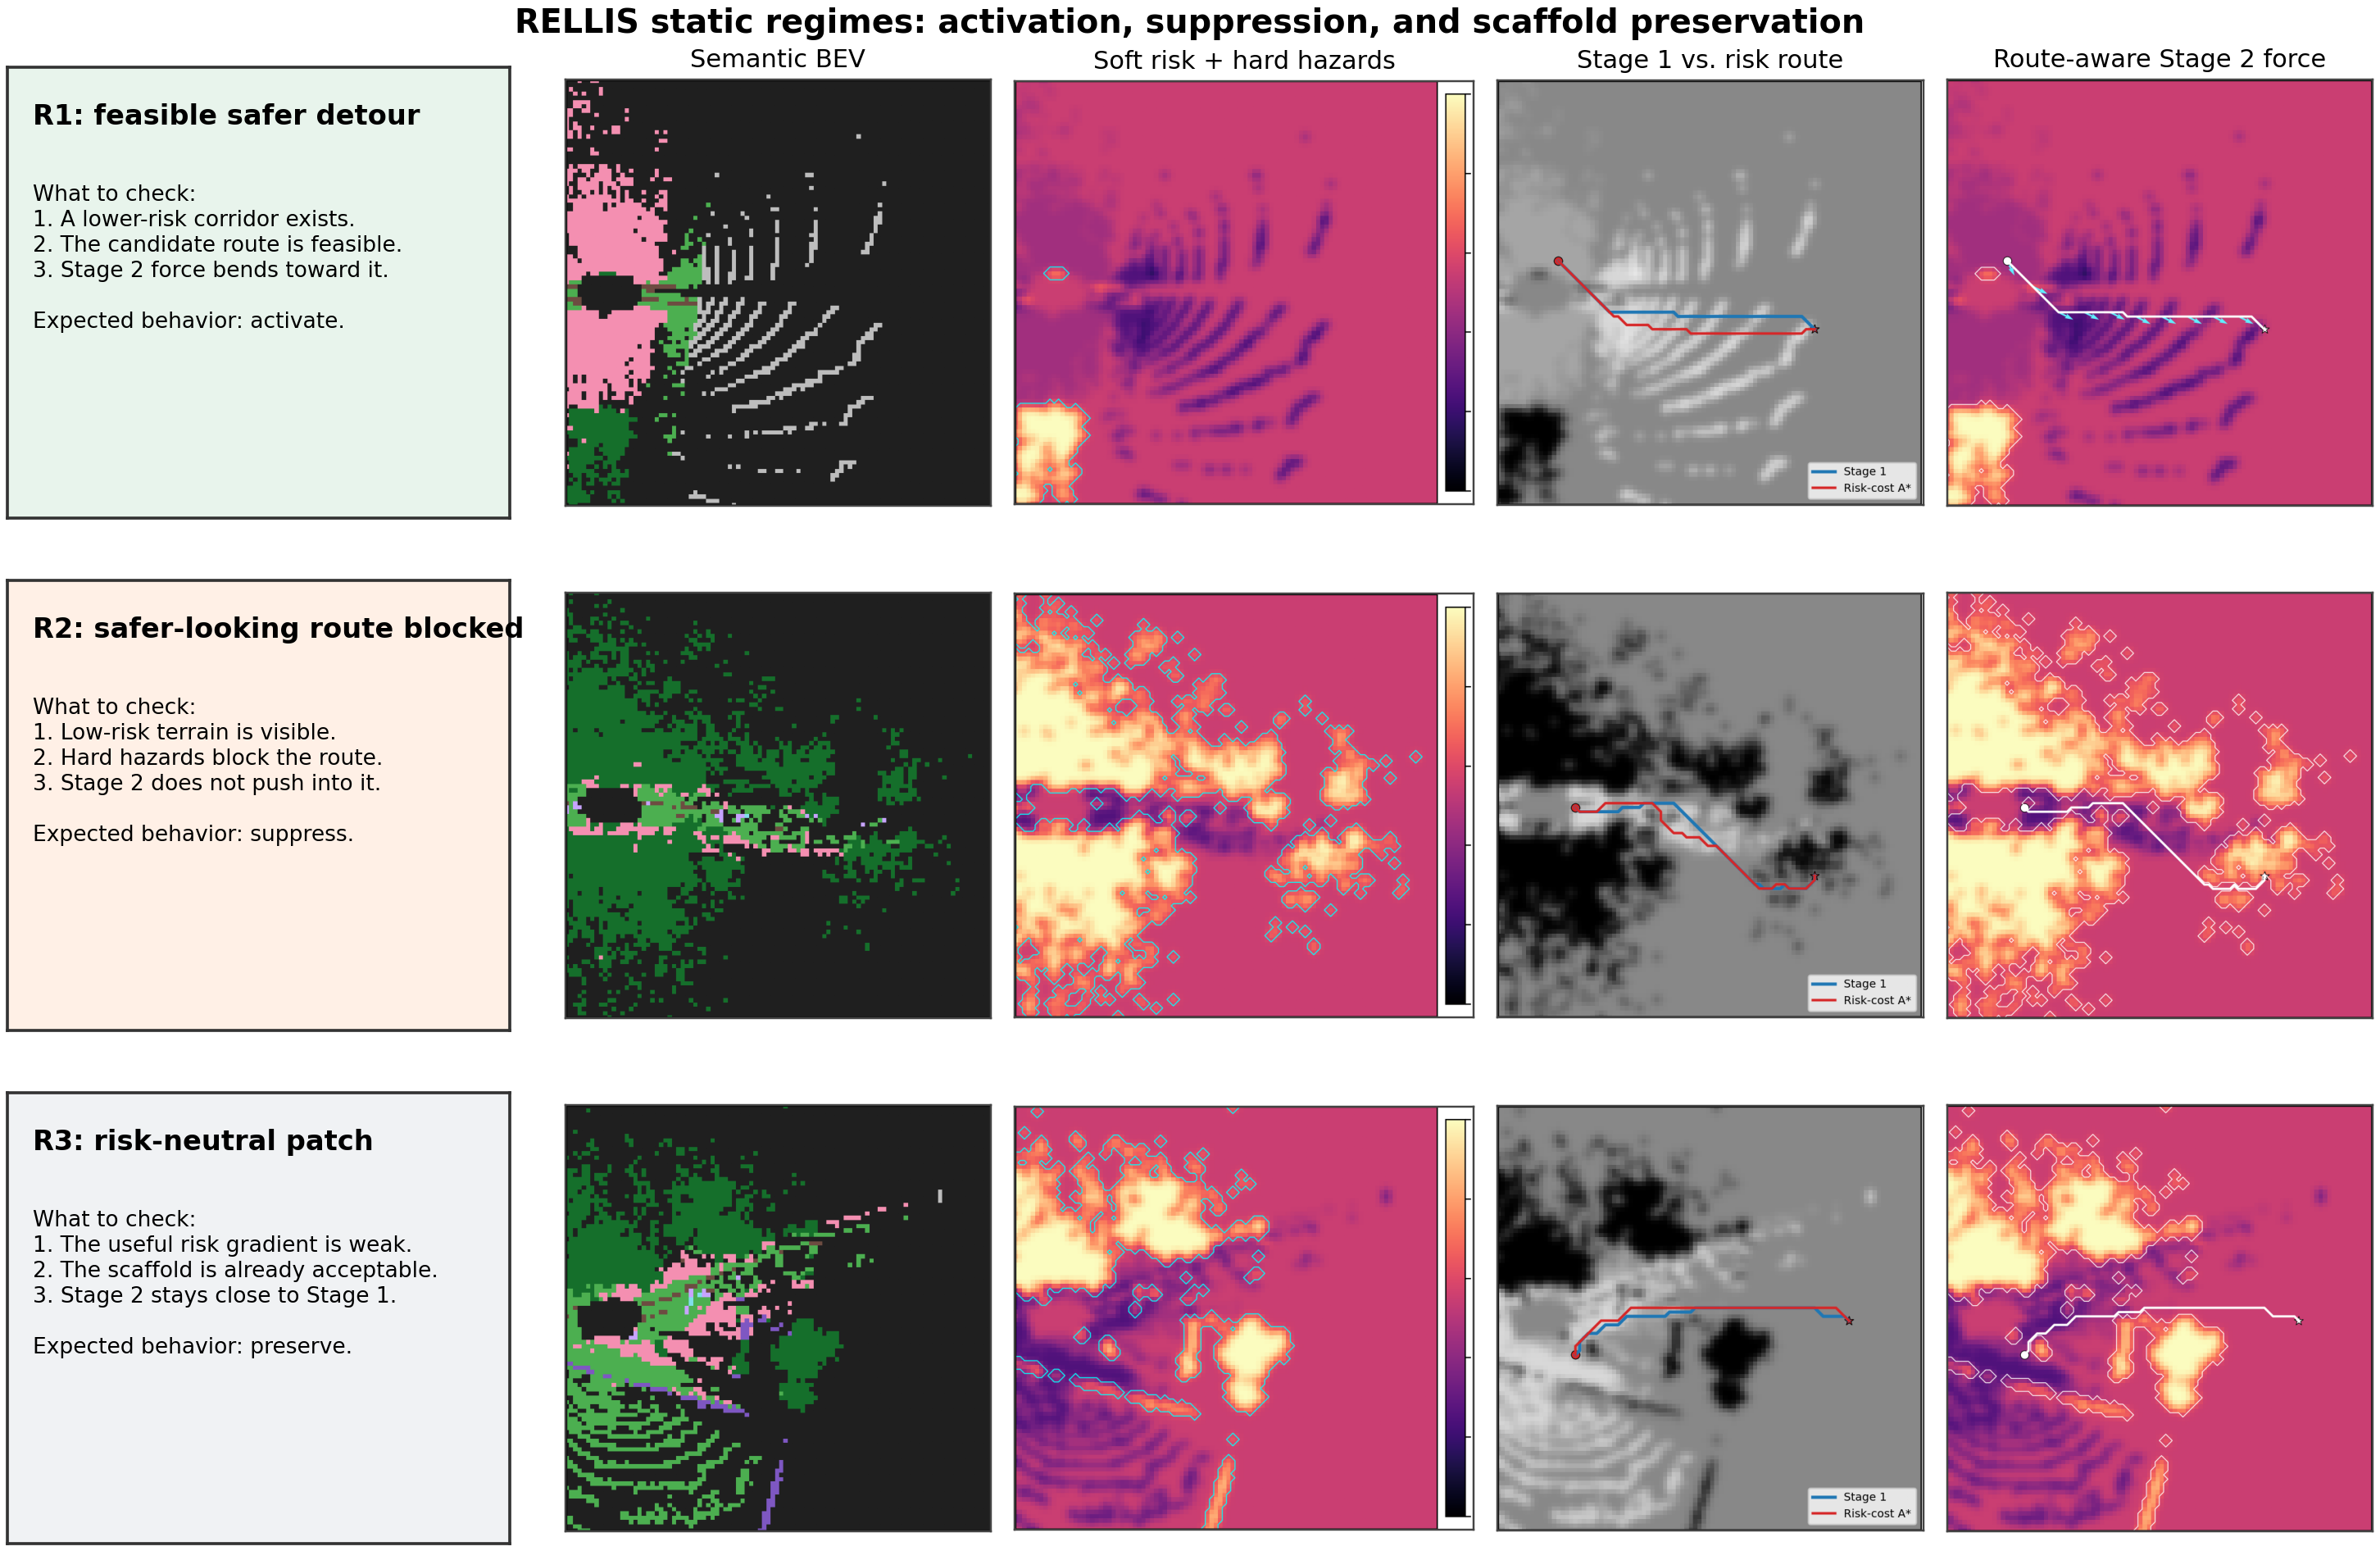
\includegraphics[width=\linewidth]{figures/rellis_static_r1r2r3_grid.png}
\caption{\textbf{RELLIS static regime panels.}
Each row shows one regime; columns give the semantic BEV, risk map,
candidate paths, and route-aware material-aware force arrows.
In R1 the force bends toward the feasible lower-risk detour.
In R2 the force is suppressed despite a locally attractive low-risk region
blocked by hard hazards.
In R3 the risk context is neutral and the material-aware policy preserves the
geometry-only policy.}
\label{fig:app_rellis_regime_panels}
\end{figure*}

\subsection{DFC2018 complete results}
\label{app:dfc_full}
Table~\ref{tab:app_dfc_main_metrics} reports the full DFC comparison including
privileged full-map planners; Table~\ref{tab:app_dfc_failure_modes} gives the
failure-mode breakdown, and Figure~\ref{fig:app_dfc_method_panels} shows the
corresponding trajectories per method on a representative episode. Full-map planners obtain lower raw static risk with
global access, while the material-aware policy repairs the geometry-only policy
with smoother trajectories and zero oscillation.

\begin{table}[htbp]
\centering
\caption{\textbf{DFC2018 full evaluation.}
Means over $300$ paired test episodes. ``Cat.\ fail'' is the fraction of
episodes with at least one hard-hazard contact; ``Osc.''\ is total absolute
heading change along the path, $\sum_t|\Delta\theta_t|$ (not curvature energy,
which squares the increments); ``Hard len.''\ is the path length traversed
inside hard hazards; and ``Fail score'' is a fixed weighted penalty combining
hard contacts, hard-hazard length, risk exposure, barrier violation, excess
path ratio, oscillation, and catastrophic failure.
\emph{Bold marks our method's row, not the best value in each column.} The
full-map planners obtain lower raw risk than any local-sensing method; our
comparison of record is against the geometry-only policy operating under the
same local-information contract, which we repair on every metric.
Oracle A$^*$ is privileged (global map access) and serves as a
reference ceiling, not a fair local-sensing competitor.}
\label{tab:app_dfc_main_metrics}
\scriptsize
\setlength{\tabcolsep}{3pt}
\renewcommand{\arraystretch}{1.08}
\resizebox{\linewidth}{!}{%
\begin{tabular}{lrrrrrrrr}
\toprule
Method & Success$\uparrow$ & Cat.\ fail$\downarrow$ & Hard len.$\downarrow$
       & Risk$\downarrow$ & Risk/m$\downarrow$ & Len.\ ratio
       & Osc.$\downarrow$ & Fail score$\downarrow$ \\
\midrule
Blind Dijkstra            & $1.000$ & $0.967$ & $55.386$ & $55.292$ & $0.244$ & $1.000$ & $1.990$  & $12927.5$ \\
Geometry-only A$^*$       & $1.000$ & $0.033$ & $0.576$  & $10.365$ & $0.042$ & $1.069$ & $24.819$ & $164.5$ \\
Risk-weighted A$^*$       & $1.000$ & $0.033$ & $0.333$  & $3.753$  & $0.014$ & $1.106$ & $54.480$ & $127.0$ \\
Oracle A$^*$$^\dagger$    & $1.000$ & $0.000$ & $0.000$  & $3.664$  & $0.014$ & $1.169$ & $58.512$ & $37.2$ \\
CVaR costmap A$^*$        & $1.000$ & $0.033$ & $0.287$  & $3.318$  & $0.012$ & $1.143$ & $72.780$ & $120.8$ \\
Chance-constrained MPC    & $1.000$ & $0.033$ & $0.287$  & $4.171$  & $0.016$ & $1.116$ & $58.957$ & $114.0$ \\
PPO-Lagrangian            & $0.800$ & $0.233$ & $0.355$  & $3.753$  & $0.014$ & $1.104$ & $13.221$ & $200.3$ \\
Geometry-only policy        & $0.867$ & $0.600$ & $21.106$ & $23.267$ & $0.099$ & $1.044$ & $82.212$ & $53216.6$ \\
\textbf{Material-aware}     & $\mathbf{1.000}$ & $\mathbf{0.100}$ & $\mathbf{0.658}$
                          & $\mathbf{9.493}$ & $\mathbf{0.039}$ & $\mathbf{1.045}$
                          & $\mathbf{7.629}$ & $\mathbf{115.8}$ \\
\bottomrule
\end{tabular}}
\end{table}

\begin{table}[htbp]
\centering
\caption{\textbf{DFC failure-mode breakdown.}
Fraction of the $300$ test episodes exhibiting each failure mode; an episode may
exhibit more than one, so rows do not sum to one.
\emph{Bold marks our method's row, not the best value in each column.}
Risk planners reduce raw material cost but frequently introduce discrete
oscillation ($0.83$--$0.90$ of episodes); the material-aware policy primarily
repairs the learned geometry-only policy, eliminating oscillation
($0.63\!\to\!0.00$) and cutting hard-hazard episodes ($0.60\!\to\!0.10$),
while remaining worse than the risk planners on high-soft-risk episodes
($0.40$ vs.\ $0.07$).}
\label{tab:app_dfc_failure_modes}
\scriptsize
\setlength{\tabcolsep}{4pt}
\renewcommand{\arraystretch}{1.08}
\begin{tabular}{lrrrrr}
\toprule
Method & No path & Hard haz. & High soft risk & Excess detour & Osc. \\
\midrule
Blind Dijkstra         & $0.00$ & $0.97$ & $0.97$ & $0.00$ & $0.00$ \\
Geometry A$^*$         & $0.00$ & $0.03$ & $0.20$ & $0.07$ & $0.43$ \\
Risk-weighted A$^*$    & $0.00$ & $0.03$ & $0.07$ & $0.10$ & $0.83$ \\
CVaR costmap A$^*$     & $0.00$ & $0.03$ & $0.07$ & $0.17$ & $0.90$ \\
Chance-const.\ MPC     & $0.00$ & $0.03$ & $0.07$ & $0.07$ & $0.83$ \\
PPO-Lagrangian         & $0.20$ & $0.23$ & $0.10$ & $0.13$ & $0.23$ \\
Geometry-only policy     & $0.13$ & $0.60$ & $0.63$ & $0.00$ & $0.63$ \\
\textbf{Material-aware}  & $\mathbf{0.00}$ & $\mathbf{0.10}$ & $\mathbf{0.40}$
                       & $\mathbf{0.03}$ & $\mathbf{0.00}$ \\
\bottomrule
\end{tabular}
\end{table}

\begin{figure*}[htbp]
\centering
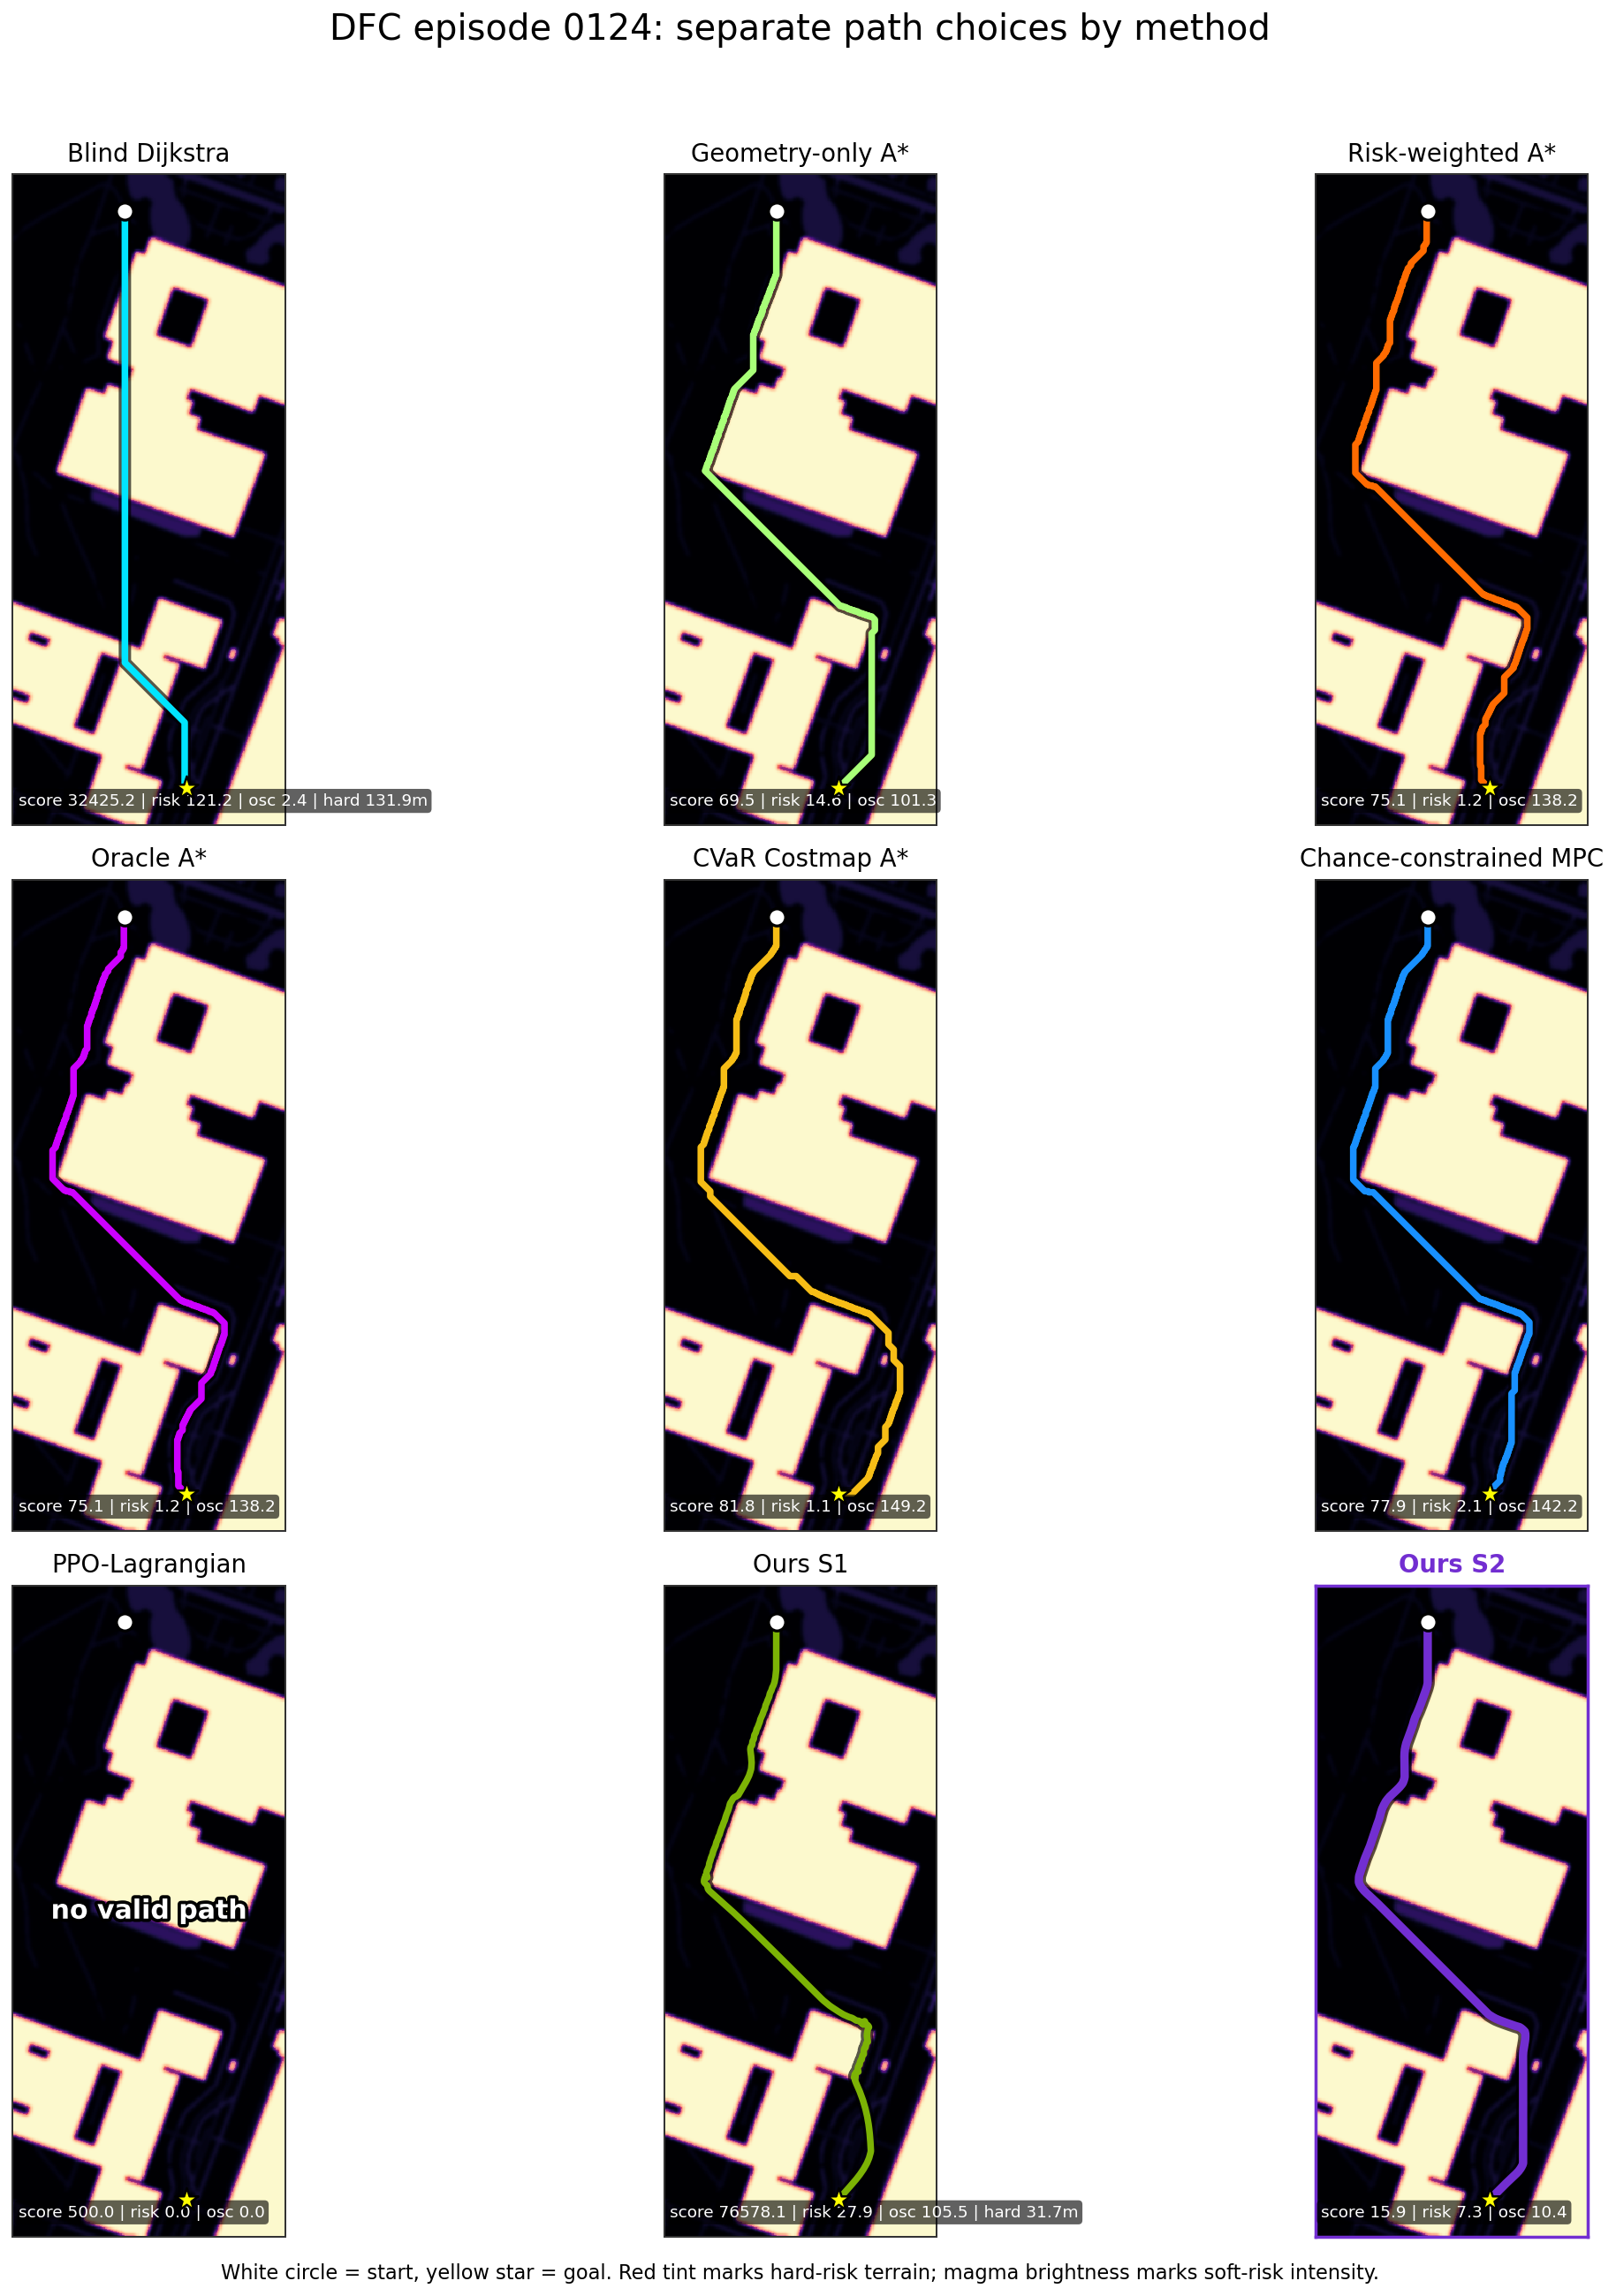
\includegraphics[width=\linewidth]{figures/dfc_ep0124_method_panels.png}
\caption{\textbf{Independent DFC path panels (episode 0124).}
Each panel shows one method's trajectory on the same episode.
The material-aware policy combines zero hard-hazard length, modest detour, and no
oscillation; discrete risk planners reduce raw risk but oscillate
heavily.}
\label{fig:app_dfc_method_panels}
\end{figure*}

\subsection{RELLIS-Dyn complete event results}
\label{app:rellis_dyn}

Table~\ref{tab:app_rellis_dyn_8event_groups} reports reaction delay and
post-event CVaR for all eight event types; the non-auditable ``wins?'' column
has been removed. DWA responds more quickly to each raw environmental change
and generally obtains lower post-event CVaR. Our advantage on this benchmark
is therefore not faster reaction, because aggregated across events the material-aware
method achieves higher success ($0.938$ vs.\ $0.566$), substantially fewer
stuck episodes ($0.111$ vs.\ $0.510$), and a lower path-length ratio
($1.038$ vs.\ $1.413$). Table~\ref{tab:app_rellis_dyn_delay_sensitivity}
shows that the reaction-delay ordering is stable across threshold $\delta$.

\begin{table}[htbp]
\centering
\caption{\textbf{RELLIS-Dyn eight-event summary} ($100$ episodes per event).
Reaction delay (steps from the event to a route deviation) and post-event
violation CVaR are reported directly; lower is better for both. We report the
unfavourable comparison in full, since DWA reacts faster on all eight events and also
attains lower post-event CVaR on all eight, so on these two axes the reactive
baseline is not dominated by our method in any event group
(Fig.~\ref{fig:app_rellis_dyn_pareto}). The material-aware field's advantage is
in \emph{when} exposure is admitted rather than how fast the route changes, as shown by
see the stale-exposure comparison in Fig.~\ref{fig:app_rellis_dyn_corridor} and
the temporal-selectivity results in Table~\ref{tab:delayed_escape}, where the
same DWA controller pre-activates on $0.95$ of episodes against our $0.38$.}
\label{tab:app_rellis_dyn_8event_groups}
\small
\setlength{\tabcolsep}{5pt}
\renewcommand{\arraystretch}{1.08}
\begin{tabular}{llcccc}
\toprule
Group & Event
  & Material delay & DWA delay
  & Material CVaR & DWA CVaR \\
\midrule
A-soft & Mud onset              & $8.2$ & $2.8$ & $0.853$ & $0.688$ \\
A-soft & Puddle expansion       & $7.9$ & $2.5$ & $0.664$ & $0.610$ \\
B-hard & Corridor closes        & $7.2$ & $3.4$ & $0.588$ & $0.551$ \\
B-hard & Corridor opens         & $5.1$ & $2.3$ & $0.561$ & $0.539$ \\
C-dyn  & Crossing obstacle      & $8.2$ & $3.2$ & $0.561$ & $0.560$ \\
C-dyn  & Moving obs.\ blocks    & $5.7$ & $4.0$ & $0.743$ & $0.601$ \\
D-comp & Mud + blocked detour   & $7.3$ & $2.7$ & $0.898$ & $0.712$ \\
D-comp & Delayed escape opens   & $5.6$ & $2.2$ & $0.859$ & $0.664$ \\
\bottomrule
\end{tabular}
\end{table}

\begin{table}[htbp]
\centering
\caption{\textbf{Reaction delay sensitivity to the detection threshold $\delta$}
(corridor-opens, $100$ episodes). Reaction delay is the number of steps from the
event until the method's response first exceeds the detection threshold
$\delta$; the delay is therefore a function of an arbitrary threshold, and this
table reports how much. Varying $\delta$ shifts the absolute delays but not
their ordering across methods, so the comparison in
Table~\ref{tab:app_rellis_dyn_8event_groups} is not an artifact of one threshold
choice. Lower is better.}
\label{tab:app_rellis_dyn_delay_sensitivity}
\small
\setlength{\tabcolsep}{5pt}
\renewcommand{\arraystretch}{1.08}
\begin{tabular}{lccc}
\toprule
$\delta$ (m) & Material-aware$\downarrow$ & DWA$\downarrow$ & Local A*$\downarrow$ \\
\midrule
$0.10$ & $5.3$ & $2.5$ & $4.8$ \\
$0.15$ & $5.1$ & $2.3$ & $4.6$ \\
$0.20$ & $4.8$ & $2.1$ & $4.3$ \\
\bottomrule
\end{tabular}
\end{table}

\begin{figure*}[htbp]
\centering

\includegraphics[width=\textwidth]{%
  figures/rellis_dyn_corridor_opens_timeline.png}
\caption{\textbf{RELLIS-Dyn corridor opens (dynamic R1).}
\emph{How to read.} the background is the soft-risk map (colorbar at right) at
the timestep printed in each panel title; white contours bound the hard
(infeasible) mask; the \textcolor{cyan}{cyan} outline marks the corridor cells
that switch from infeasible to feasible at $t_{\rm event}$, which is the event itself.
Green is the material-aware policy (Stage 2), blue is DWA; dots mark the pose at
that timestep and arrows the movement force.
\emph{What to see.} the corridor is sealed in A and open from B onward. The
material-aware field reshapes toward the newly feasible low-risk corridor and
enters it (panel D), while DWA continues along its prior route and reaches the
corridor later. The bottom trace is soft risk on the executed cell (axis zoomed
to the data range); the shaded gap between the curves is the stale exposure DWA
accumulates, quantified in the panel title (stale exposure $0.00$ vs $1.69$;
path-length ratio $1.020$ vs $1.107$).
\emph{How representative.} across the 100 corridor-opens episodes, the
material-aware policy routes into the opened corridor in 59; episode 13 is shown
because it separates the two methods cleanly. Aggregate results over all
episodes are in Table~\ref{tab:app_rellis_dyn_8event_groups}.}
\label{fig:app_rellis_dyn_corridor}
\end{figure*}

\begin{figure*}[htbp]
\centering

\includegraphics[width=0.82\textwidth]{%
  figures/rellis_dyn_8event_group_pareto.png}
\caption{\textbf{RELLIS-Dyn 8-event group Pareto.}
One panel per event group; each marker is one method averaged over that group's
events. The $x$-axis is reaction delay in steps and the $y$-axis is post-event
violation CVaR, with lower better on both. Marker colour encodes the method and
marker area the control latency in ms/step, with a key at the bottom. Stars mark the non-dominated (Pareto-optimal)
points within each panel.
\emph{What to see.} on these two axes DWA semantic is non-dominated in all four
groups, because it reacts fastest to the raw environmental change and attains the
lowest post-event CVaR, consistent with
Table~\ref{tab:app_rellis_dyn_8event_groups}. The material-aware policy attains
CVaR comparable to the replanning baselines (Local A*, Oracle) at roughly half
their reaction delay and at zero replanning latency ($0$ vs.\ $315$ and
$2{,}300$\,ms/step), but it is not Pareto-optimal in this projection. The
advantage of the witness gate is in \emph{when} exposure is admitted, through stale
exposure and temporal selectivity (Fig.~\ref{fig:app_rellis_dyn_corridor} and
Table~\ref{tab:app_rellis_dyn_delay_sensitivity}), which these two axes do
not measure.}
\label{fig:app_rellis_dyn_pareto}
\end{figure*}

\begin{figure*}[htbp]
\centering

\includegraphics[width=0.9\textwidth]{%
  figures/rellis_dyn_force_decomposition.png}
\caption{\textbf{RELLIS-Dyn force-channel decomposition.}
Channel proxies evaluated at the executed cell and averaged over rollouts of the
material-aware policy, grouped by the eight event types. The material proxy is
the risk-map gradient magnitude $\|\nabla\tilde r\|$, and the hazard proxy is
the hard-SDF gradient magnitude $\|\nabla\phi\|$ weighted by a sigmoid on the
clearance margin. These are field quantities the two channels respond to, not
the applied forces themselves (which additionally carry $\lambda_s$,
$\lambda_h$, and the gate $g$), and so are not a causal decomposition of the
resulting motion. The channels
separate as intended, since soft events (mud, puddle) drive $f_{\rm mat}$ alone,
while hard-boundary and compound events additionally drive $f_{\rm haz}$, which is
evidence that the two channels respond to the risk type they were defined for
rather than acting as one undifferentiated force.}
\label{fig:app_rellis_dyn_force_decomp}
\end{figure*}

\subsection{Highway-env complete results}
\label{app:highway_full}
Table~\ref{tab:app_highway_mechanism} is the channel-level mechanism ablation;
Tables~\ref{tab:app_highway_baselines} and~\ref{tab:app_highway_scenarios} give
the broad baseline comparison and scenario-level results, and
Figure~\ref{fig:app_highway_path_panels} shows the executed trajectories in the
three highway scenarios. MOBIL-IDM is the domain-engineered ceiling; the
material-aware field is the strongest learned method.

\begin{table}[htbp]
\centering
\caption{\textbf{Highway mechanism ablation} ($200$ paired seeds). Each row
removes or isolates one force channel, holding seeds and traffic fixed.
Columns group by scenario, covering default traffic (off-road rate), a slow leader
(collision rate, success rate), and boxed-in traffic where no lateral escape
exists (collision, off-road, mean speed). Arrows give the preferred direction.
The full channel set is needed to pass the lateral maneuver \emph{and} reject
it when the escape is removed; either channel alone fails one of the two.}
\label{tab:app_highway_mechanism}
\scriptsize\setlength{\tabcolsep}{3pt}\renewcommand{\arraystretch}{1.08}
\resizebox{\linewidth}{!}{%
\begin{tabular}{lrrrrrr}
\toprule
Variant & Def.off-rd$\downarrow$ & Slow coll$\downarrow$ & Slow succ$\uparrow$
        & Boxed coll$\downarrow$ & Boxed off-rd$\downarrow$ & Boxed spd$\uparrow$ \\
\midrule
No lateral channel     & $0.00$ & $1.00$ & $0.00$ & $1.00$ & $0.00$ & $22.33$ \\
Lateral only           & $0.20$ & $0.00$ & $1.00$ & $1.00$ & $0.00$ & $22.33$ \\
\textbf{Lateral + TTC} & $\mathbf{0.00}$ & $\mathbf{0.00}$ & $\mathbf{1.00}$
                       & $\mathbf{0.00}$ & $\mathbf{0.00}$ & $\mathbf{7.57}$ \\
\bottomrule
\end{tabular}}
\end{table}

\begin{table}[!htbp]
\centering
\caption{\textbf{Broad highway baseline comparison.}
Mean over three scenarios, $200$ seeds each. Rank is by a safety-first
lexicographic order (collision, then off-road, then risk, then speed) over all
$13$ methods evaluated; the nine shown are a representative selection, so the
printed ranks are not consecutive.
\emph{Bold marks our method's row; bold on the MOBIL-IDM row marks the two
columns it leads outright.} The material-aware policy is the strongest learned
policy, since it is the only learned method with zero collisions and zero off-road.
MOBIL-IDM is the strongest overall and should be read as a
domain-engineered ceiling. Our speed ($18.86$) is not the highest in the column, because
the faster learned policies (PPO-Lagrangian $24.61$, SAC $22.56$, geometry-only
$23.66$) achieve it by driving unsafely, at collision rates of
$0.25$--$0.68$.}
\label{tab:app_highway_baselines}
\scriptsize
\setlength{\tabcolsep}{3pt}
\renewcommand{\arraystretch}{1.08}
\resizebox{\linewidth}{!}{%
\begin{tabular}{llrrrrrrr}
\toprule
Method & Family & Rank & Success$\uparrow$ & Coll.$\downarrow$
       & Off-rd.$\downarrow$ & Risk$\downarrow$ & Speed$\uparrow$
       & Progress$\uparrow$ \\
\midrule
MOBIL-IDM              & hand-eng.      & $1/13$ & $1.00$ & $0.00$ & $0.00$ & $\mathbf{5.81}$  & $21.29$ & $\mathbf{254.8}$ \\
Risk-aware MPC         & planning       & $2/13$ & $1.00$ & $0.00$ & $0.00$ & $17.54$ & $13.75$ & $164.0$ \\
Chance-const.\ MPC     & planning       & $3/13$ & $1.00$ & $0.00$ & $0.00$ & $18.34$ & $14.79$ & $176.6$ \\
\textbf{Material-aware}  & learned field  & $\mathbf{4/13}$ & $\mathbf{1.00}$ & $\mathbf{0.00}$ & $\mathbf{0.00}$ & $18.35$ & $\mathbf{18.86}$ & $225.8$ \\
CBF-QP filter          & safety filter  & $5/13$ & $1.00$ & $0.00$ & $0.00$ & $30.66$ & $14.63$ & $175.2$ \\
IDM                    & hand-eng.      & $6/13$ & $1.00$ & $0.00$ & $0.00$ & $33.18$ & $14.08$ & $168.6$ \\
PPO-Lagrangian         & learned const. & $7/13$ & $0.75$ & $0.25$ & $0.73$ & $5.01$  & $24.61$ & $105.6$ \\
SAC                    & learned RL     & $8/13$ & $0.62$ & $0.38$ & $0.38$ & $15.12$ & $22.56$ & $160.7$ \\
Geometry-only policy     & geom.-only     & $10/13$& $0.32$ & $0.68$ & $0.32$ & $6.88$  & $23.66$ & $125.9$ \\
\bottomrule
\end{tabular}}
\end{table}

\begin{table}[htbp]
\centering
\caption{\textbf{Highway full scenario-level results.}
$200$ paired seeds per scenario, each pairing the geometry-only policy against
the material-aware policy on identical traffic. \emph{Here bold marks the best
value in each column within a scenario} (contrast
Table~\ref{tab:app_highway_baselines}, where bold marks our row); our speed in
the default scenario is not bolded because the geometry-only policy is faster
there, at a $0.95$ off-road rate. The material-aware policy changes behaviour
when the escape is useful and suppresses it when boxed, visible as the lane-change
count going to zero in the boxed scenario. See the mechanism ablation
(Table~\ref{tab:app_highway_mechanism}) for the channel-level explanation and
Figure~\ref{fig:app_highway_path_panels} for the trajectories.}
\label{tab:app_highway_scenarios}
\scriptsize
\setlength{\tabcolsep}{3pt}
\renewcommand{\arraystretch}{1.08}
\resizebox{\linewidth}{!}{%
\begin{tabular}{llrrrrrr}
\toprule
Scenario & Method & Coll.$\downarrow$ & Off-rd.$\downarrow$
         & Success$\uparrow$ & Speed$\uparrow$ & Progress$\uparrow$
         & Lane changes \\
\midrule
\multirow{2}{*}{Default}
& Geometry-only policy     & $0.05$ & $0.95$ & $0.95$ & $23.56$ & $142.95$ & $0.95$ \\
& \textbf{Material-aware}  & $\mathbf{0.00}$ & $\mathbf{0.00}$ & $\mathbf{1.00}$ & $22.66$ & $\mathbf{271.78}$ & $\mathbf{0.00}$ \\
\midrule
\multirow{2}{*}{Slow leader}
& Geometry-only policy     & $1.00$ & $0.00$ & $0.00$ & $23.79$ & $44.54$  & $0.00$ \\
& \textbf{Material-aware}  & $\mathbf{0.00}$ & $\mathbf{0.00}$ & $\mathbf{1.00}$ & $\mathbf{26.21}$ & $\mathbf{313.94}$ & $\mathbf{1.00}$ \\
\midrule
\multirow{2}{*}{Slow leader boxed}
& Geometry-only policy     & $0.00$ & $1.00$ & $1.00$ & $\mathbf{13.25}$ & $74.48$  & $1.00$ \\
& \textbf{Material-aware}  & $\mathbf{0.00}$ & $\mathbf{0.00}$ & $\mathbf{1.00}$ & $7.57$ & $\mathbf{90.19}$ & $\mathbf{0.00}$ \\
\bottomrule
\end{tabular}}
\end{table}

\begin{figure}[htbp]
\centering
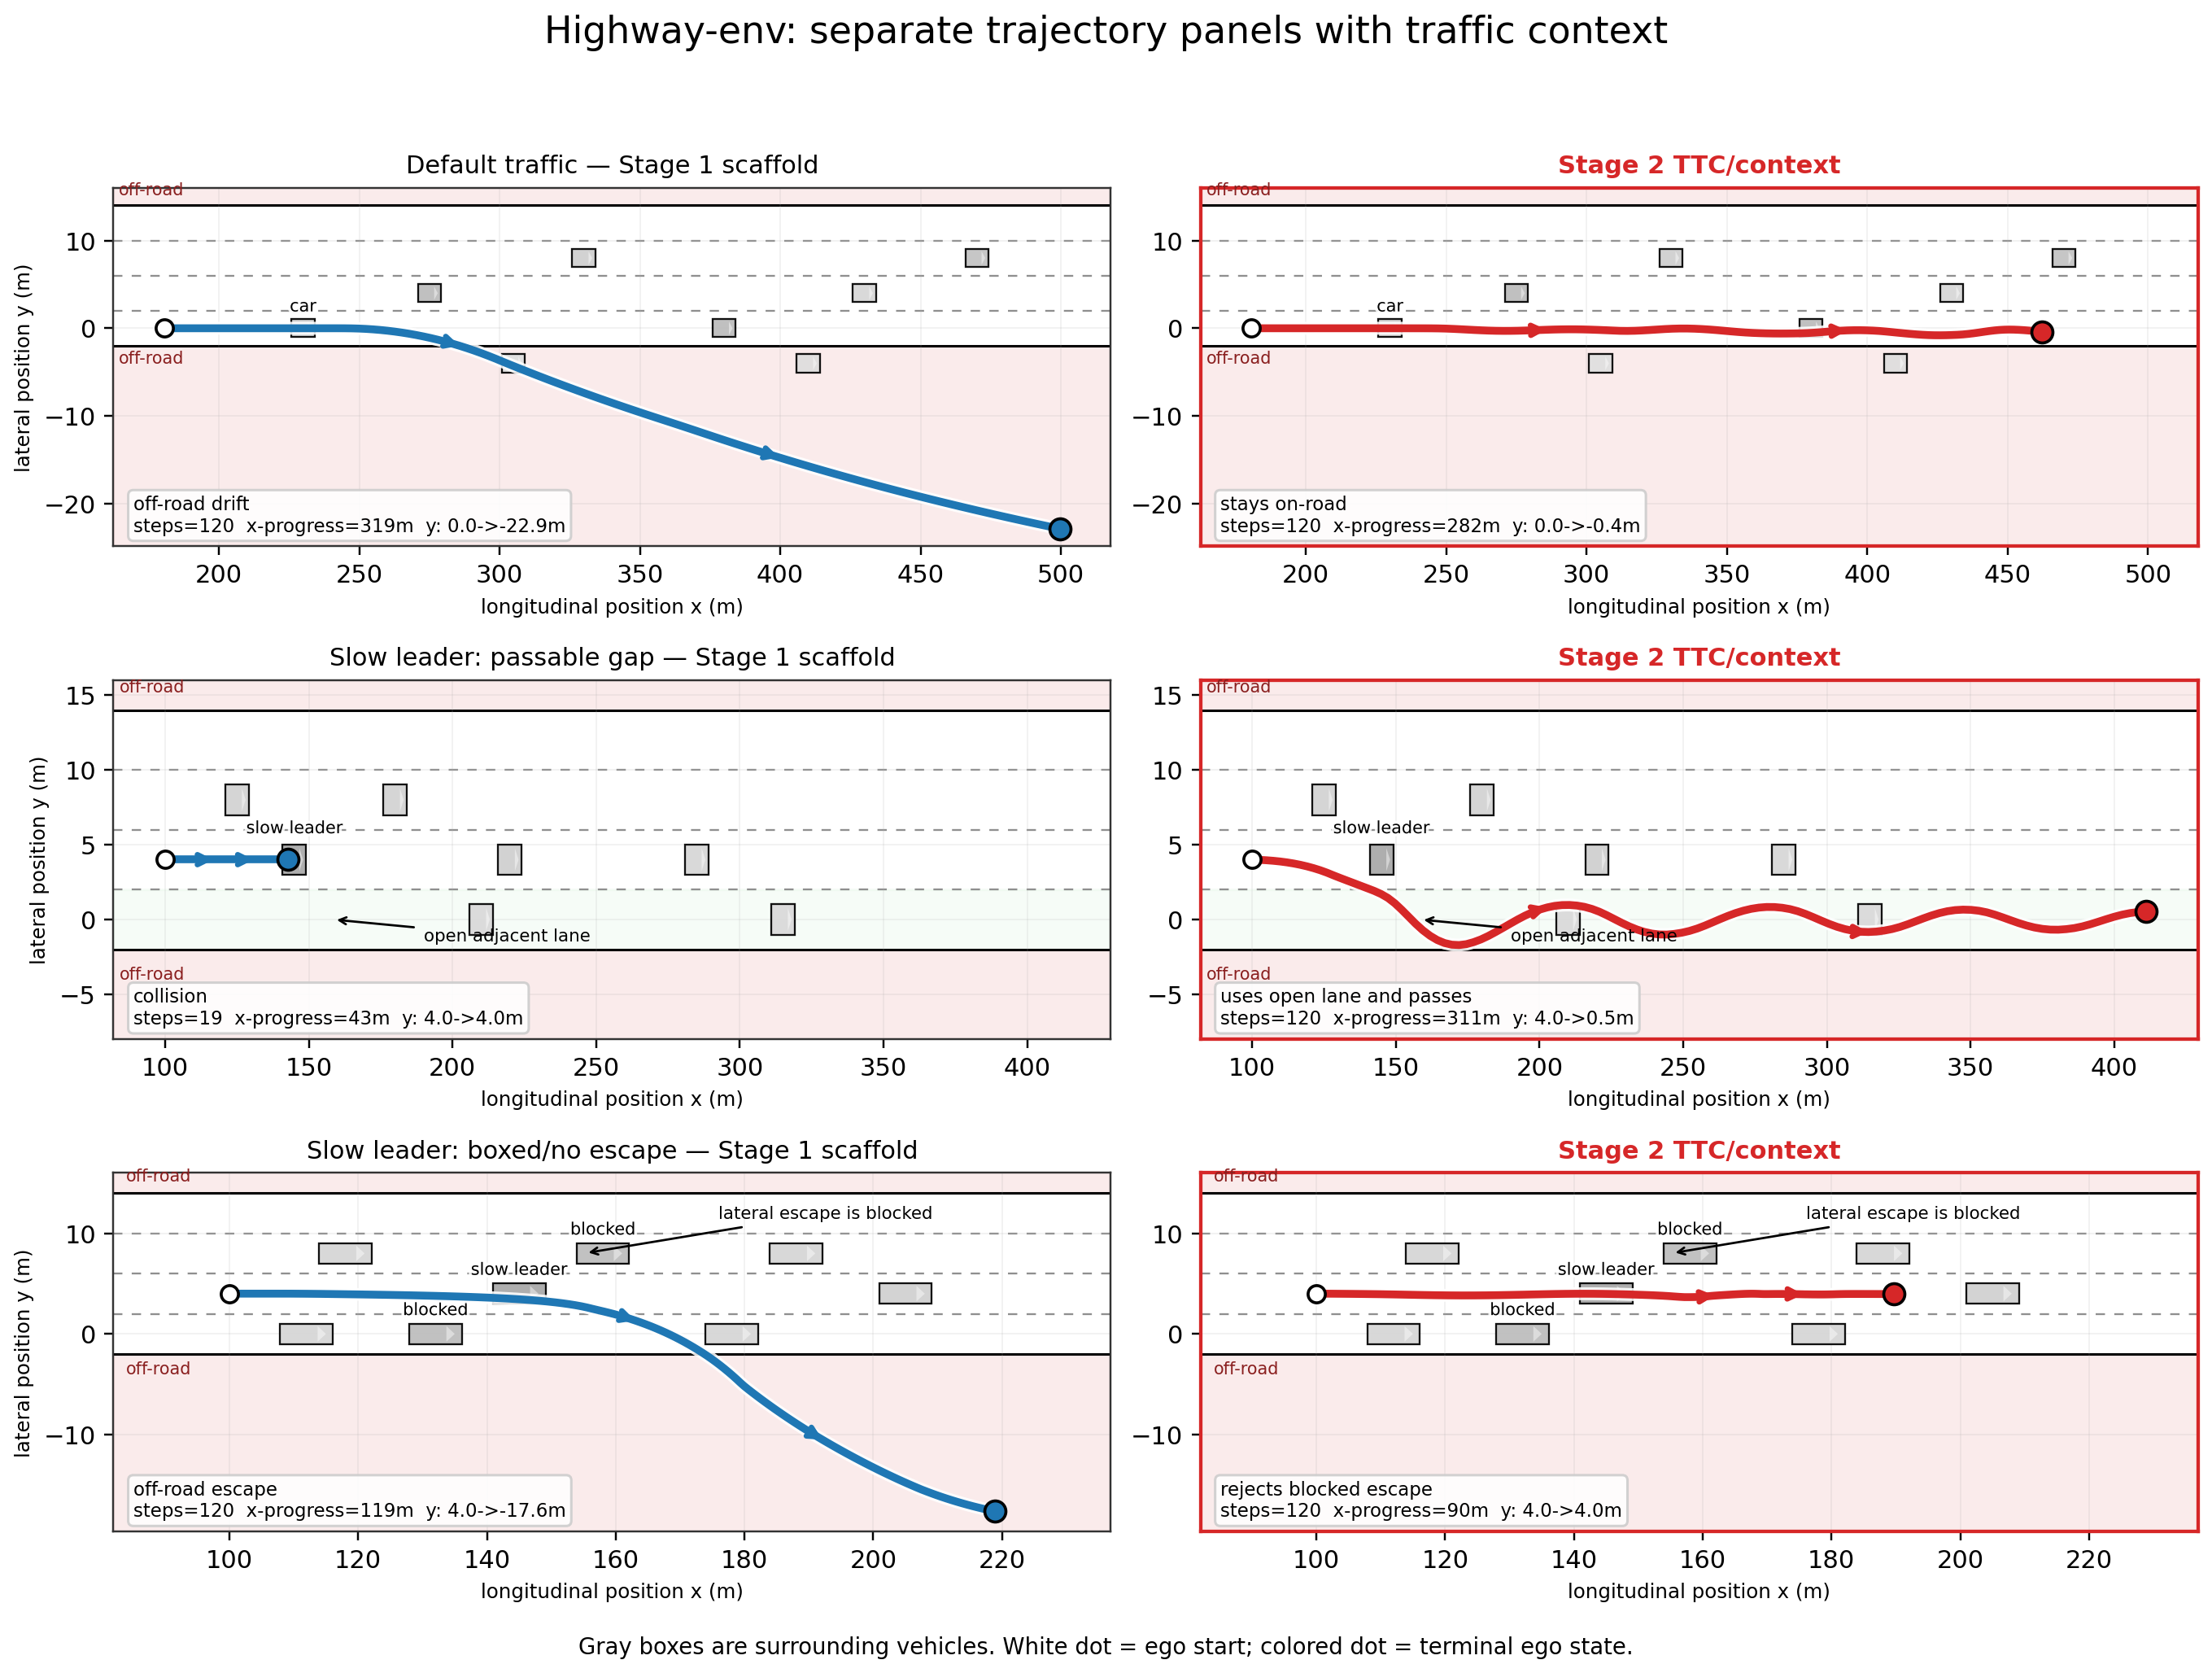
\includegraphics[width=\textwidth]{figures/highway_scenario_path_panels.png}
\caption{\textbf{Highway trajectory panels.}
Executed trajectories in the three highway-env scenarios (default traffic, slow
leader with an open adjacent lane, and boxed traffic in which no lateral escape
exists), one panel per scenario on a matched seed. The material-aware policy
stays centred in default traffic, passes the slow leader when the adjacent lane
is open, and rejects the lateral manoeuvre when boxed traffic removes the
escape, which is the same activation/suppression split quantified in
Table~\ref{tab:app_highway_scenarios}.}
\label{fig:app_highway_path_panels}
\end{figure}
\subsection{Research-question summary figures}
\label{app:rq_figures} 

\begin{figure*}[htbp]
\centering
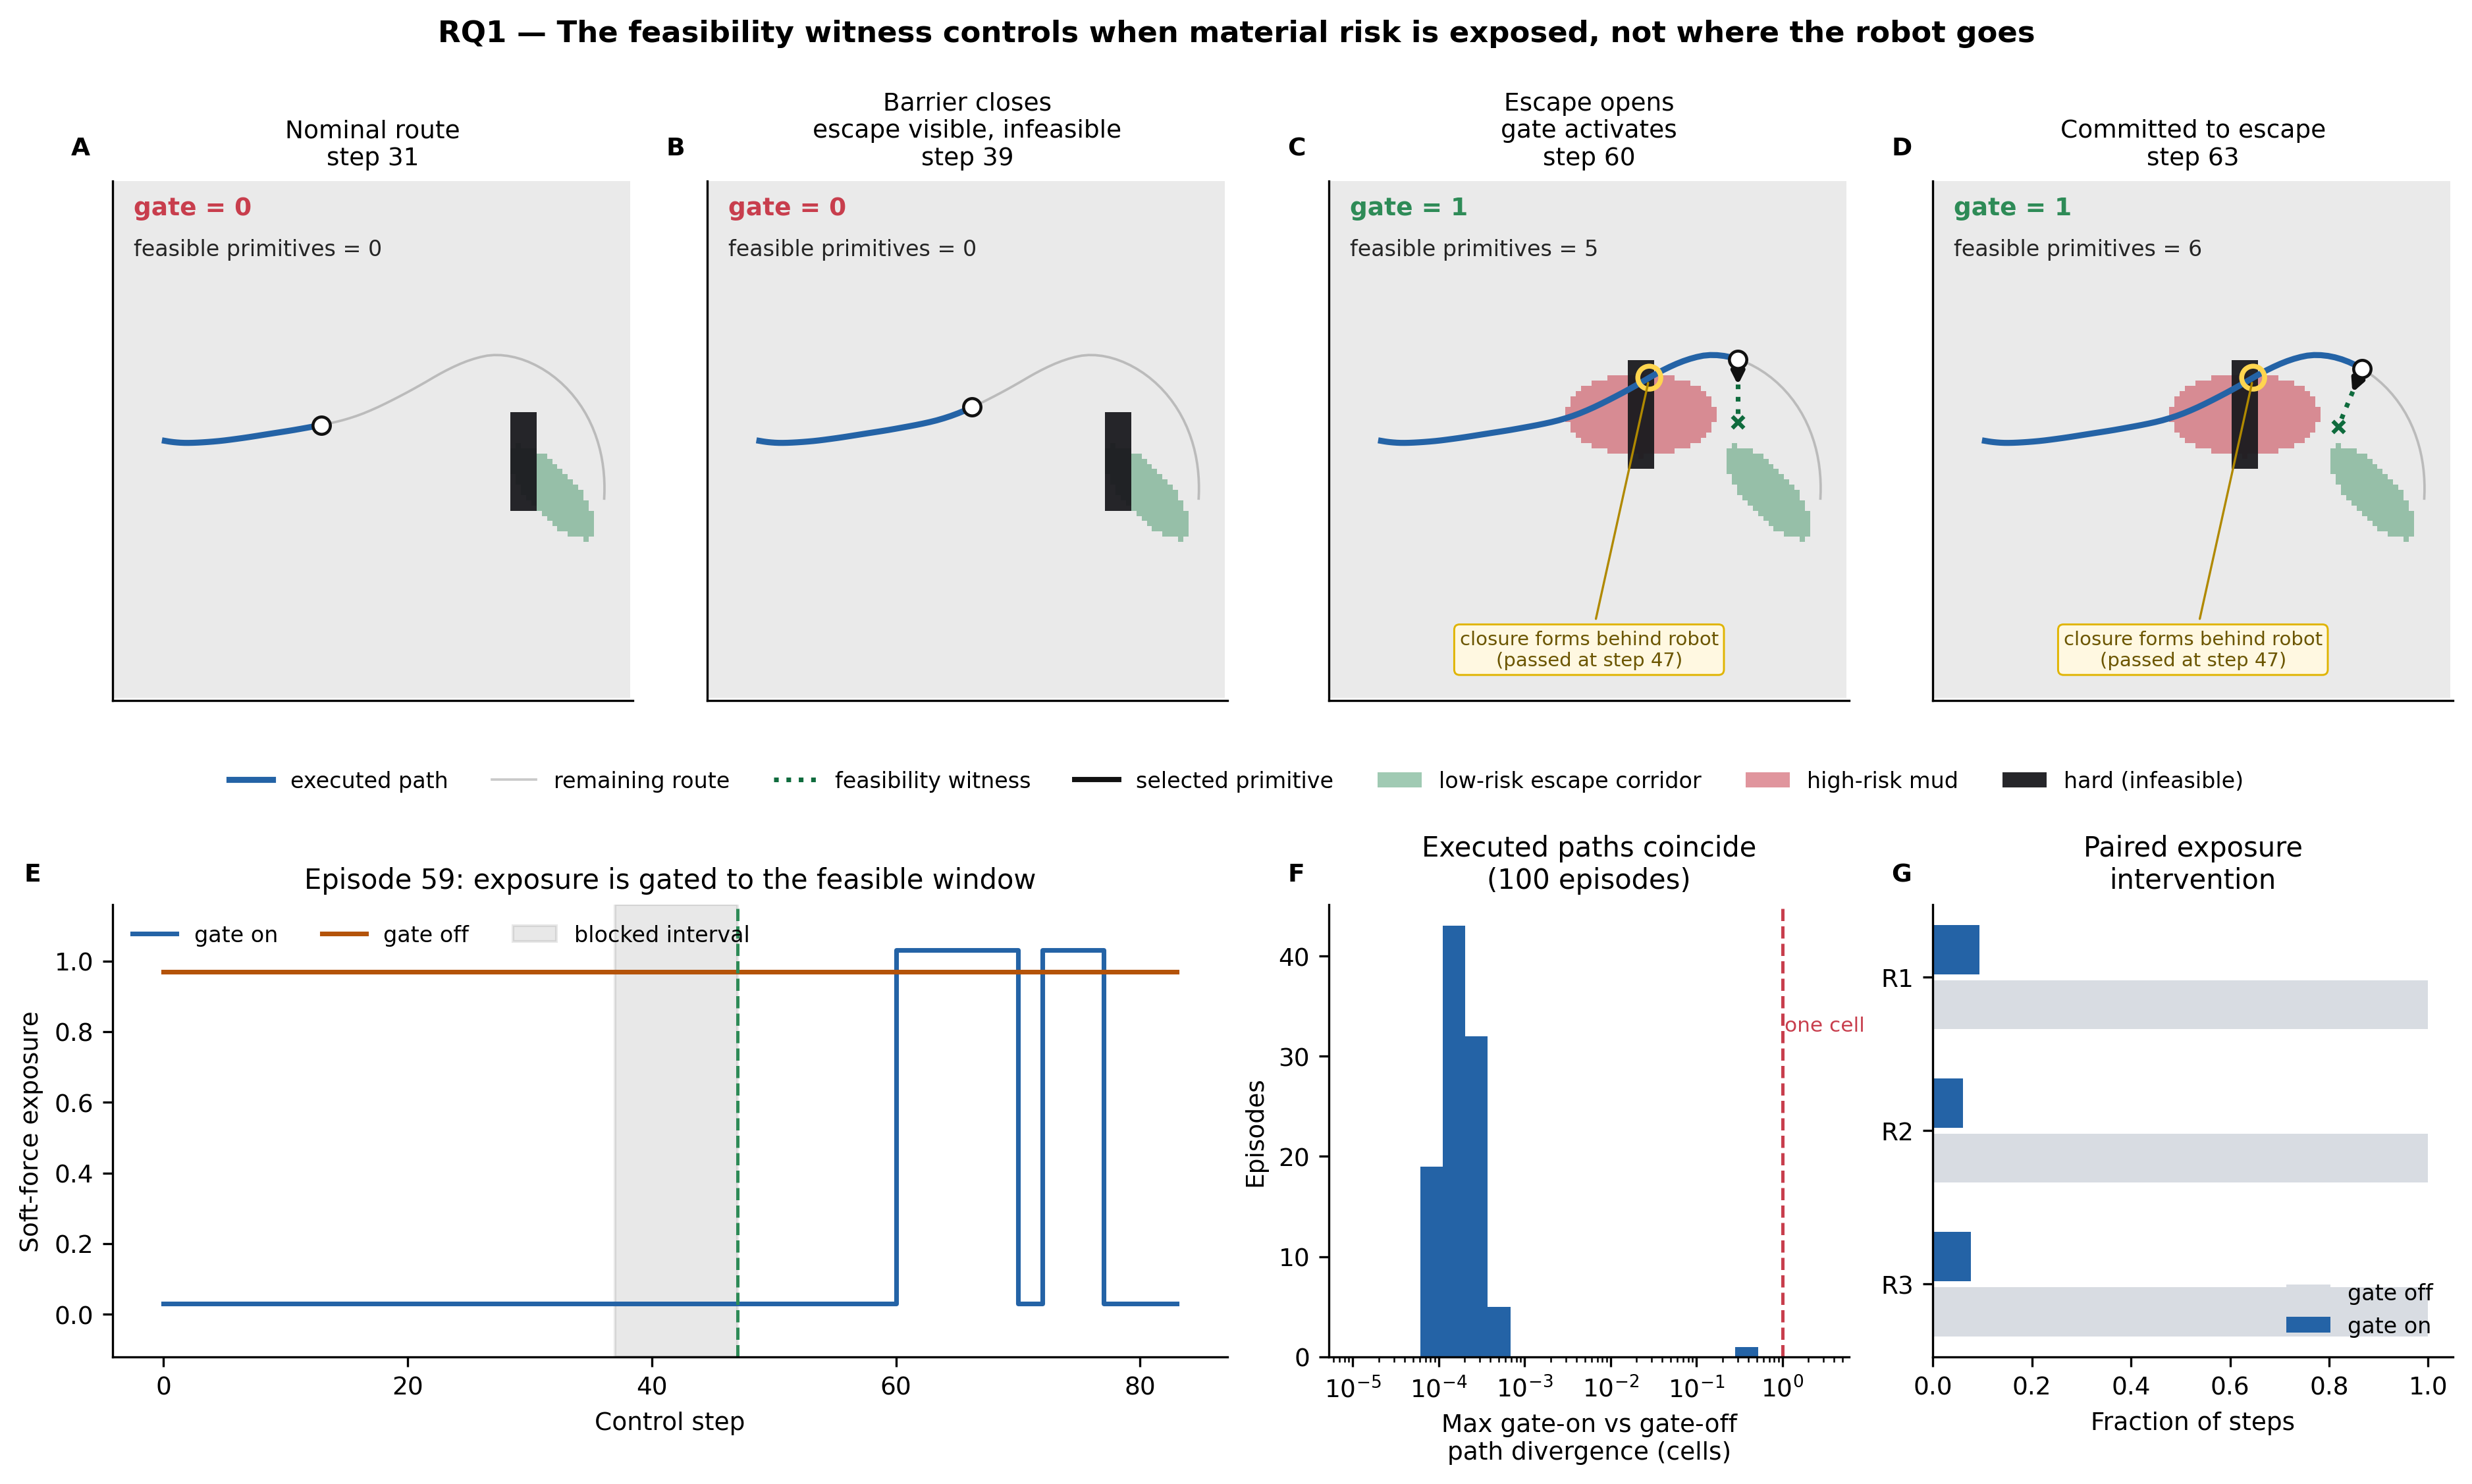
\includegraphics[width=\textwidth]{figures/rq1_gate_exposure.png}
\caption{\textbf{(RQ1) The witness gate controls \emph{when} material risk is
exposed, not \emph{where} the robot drives.}
\emph{A--D.} one delayed-required-escape rollout (episode 59) over the
reconstructed event field; blue is the executed path, grey the remainder of the
route, dotted green the feasibility witness ray, black the selected primitive.
Green shading is the low-risk escape corridor, red the high-risk mud, black the
hard (infeasible) mask. The escape corridor is visible but infeasible while the
barrier is closed (A--B, gate${=}0$, zero feasible primitives); when it opens
the gate activates and the robot commits (C--D). The closure that seals the
nominal route forms \emph{behind} the robot at the opening instant, which is why
the path appears to cross it.
\emph{E.} soft-force exposure over time for the same episode with the gate on
and off. \emph{F.} the two arms execute the same path, since across all $100$
paired episodes the maximum gate-on/gate-off divergence is $0.33$ cells (median
$2\times10^{-4}$), so the gate modulates exposure, not route.
\emph{G.} paired exposure by regime ($0.094/0.061/0.076$ with the gate on vs.\
$1.000$ off), matching Table~\ref{tab:gate_toggle}.
Scene-dependent base risk is not recoverable from the saved artifacts, so only
the event-induced structure is drawn; it is shown as labelled categorical
layers rather than an invented continuous risk map.}
\label{fig:rq1}
\end{figure*}

\begin{figure*}[htbp]
\centering
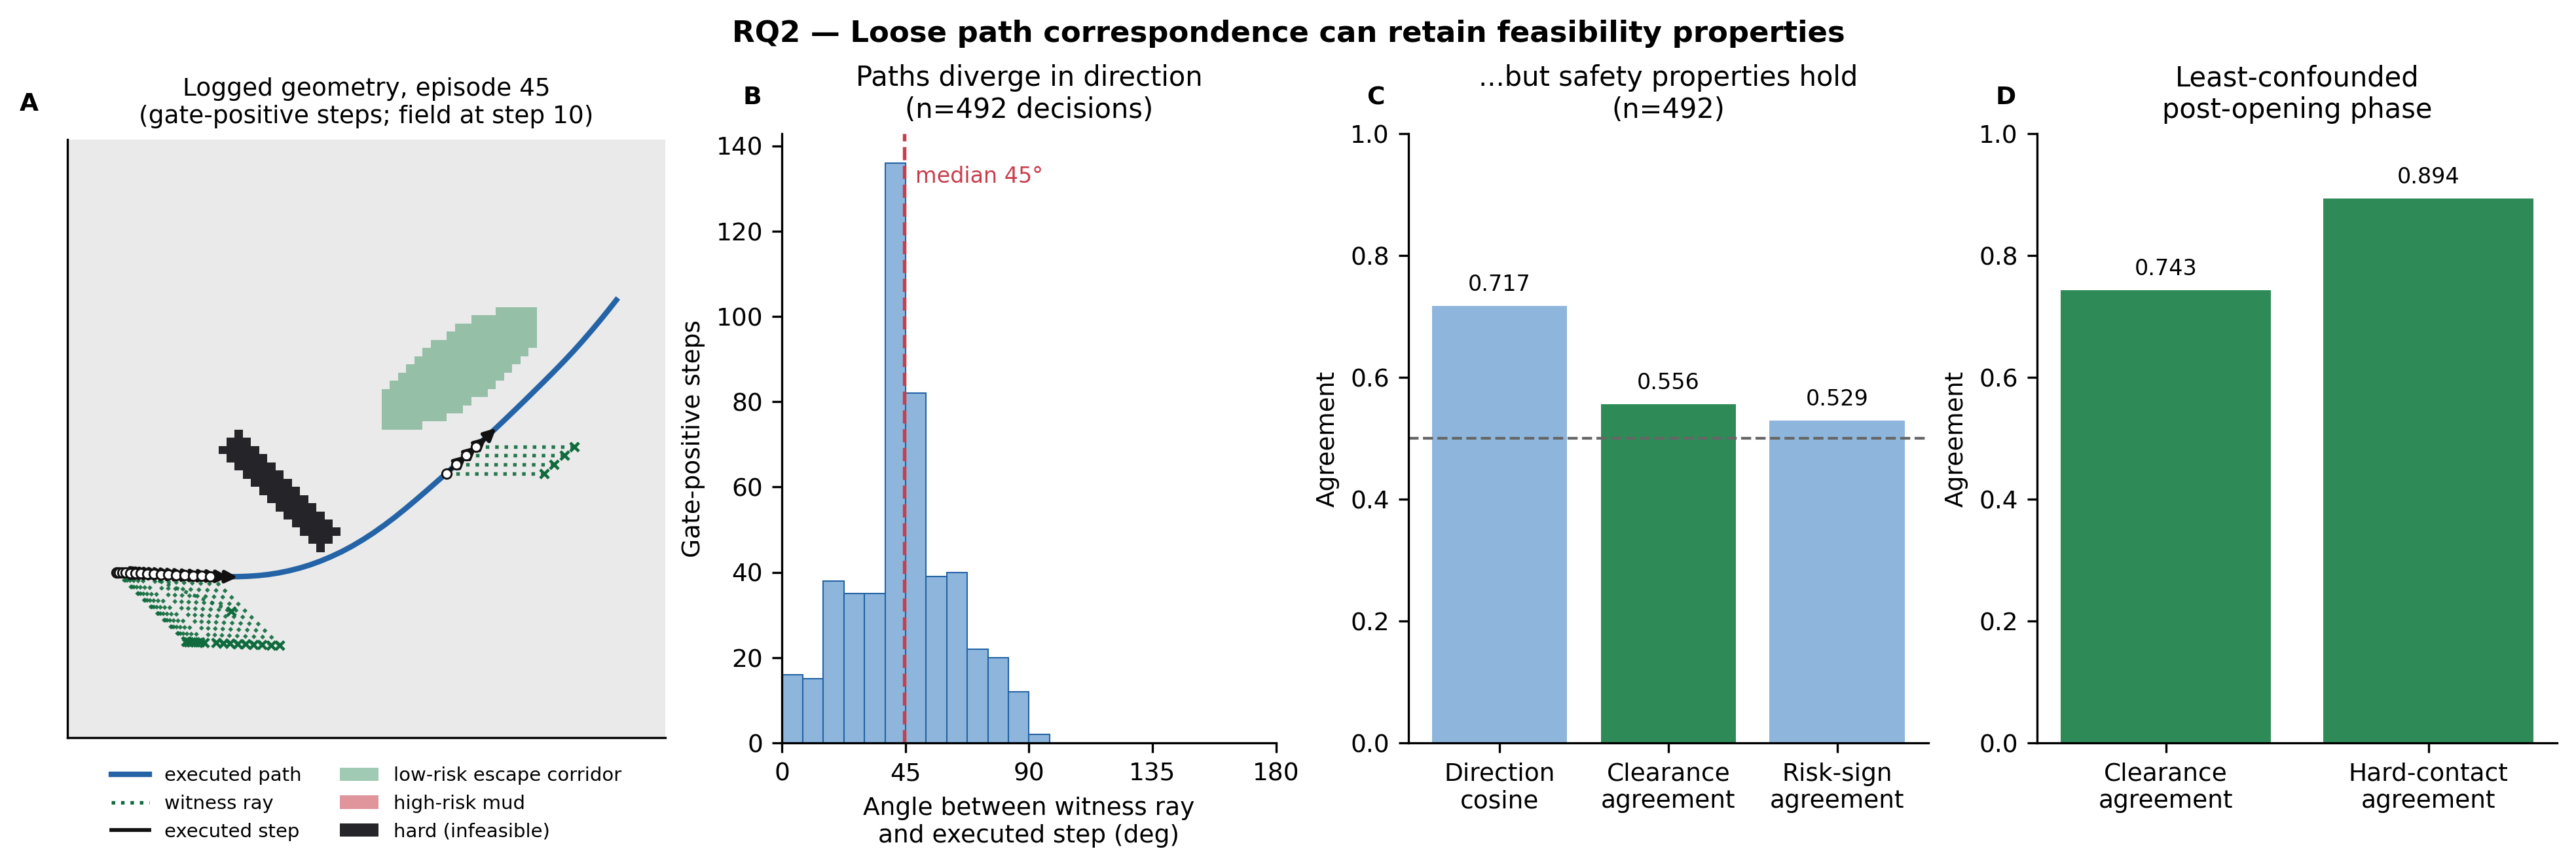
\includegraphics[width=\textwidth]{figures/rq2_witness_execution.png}
\caption{\textbf{(RQ2) Loose path correspondence, preserved feasibility
properties.}
\emph{A.} logged geometry at every gate-positive step of one episode, where the
witness rays (dotted green) fan away from the executed path (blue), confirming
$k^\star$ is not tracked. \emph{B.} over all $492$ activations the angle between
the witness ray and the executed step has median $45^\circ$.
\emph{C.} despite that, safety-relevant properties transfer, with median direction
cosine $0.717$, clearance agreement $0.556$, risk-sign agreement $0.529$ over
the full episode. \emph{D.} in the post-opening phase, where the feasibility
signal is least temporally confounded, clearance agreement is $0.743$ and
hard-contact agreement $0.894$. Numbers match
Table~\ref{tab:witness_validity}.}
\label{fig:rq2}
\end{figure*}

\begin{figure*}[htbp]
\centering
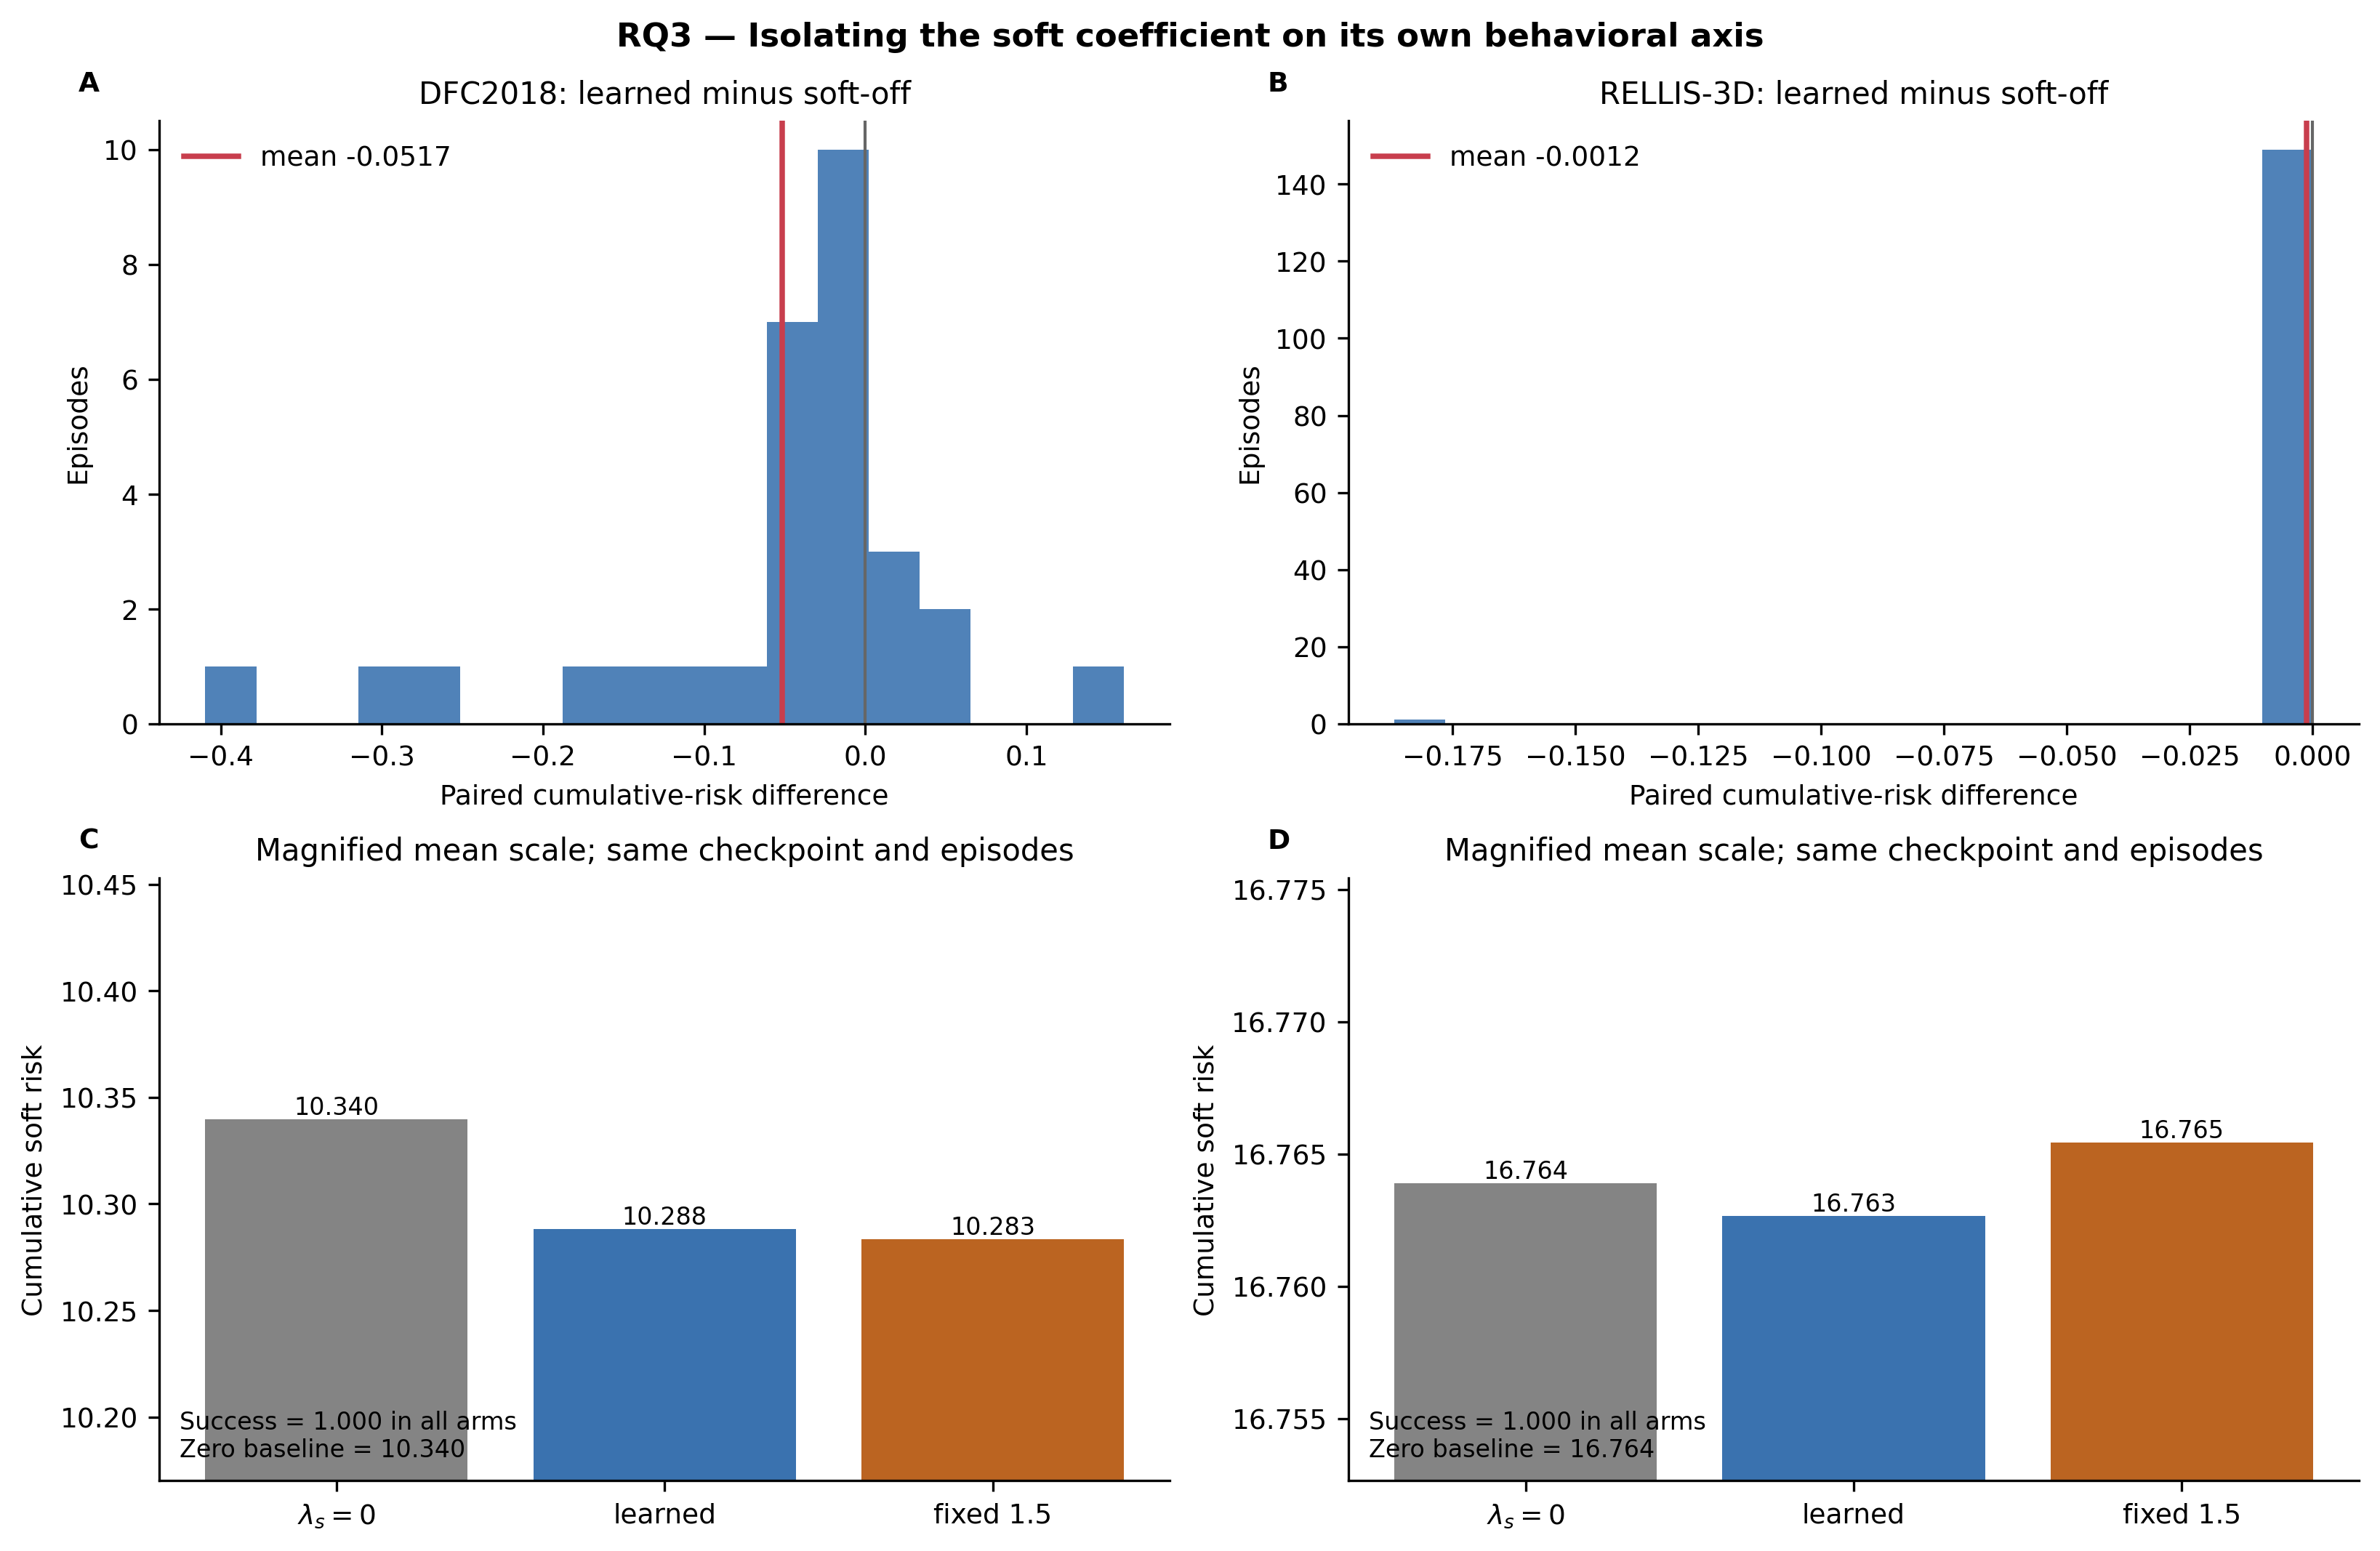
\includegraphics[width=\textwidth]{figures/rq3_isolated_soft_channel.png}
\caption{\textbf{(RQ3) The material channel acts where the material field is
informative and is near-silent where it is not.}
This is a one-factor intervention in which $\lambda_s$ is varied with $\lambda_h$, the gate, the
checkpoint, and the episodes all held fixed.
\emph{A--B.} paired per-episode cumulative-risk differences (learned minus
soft-off) for DFC2018 (mean $-0.052$) and RELLIS-3D (mean $-0.001$).
\emph{C--D.} the same comparison as group means on a magnified scale, giving
DFC2018 $10.340\!\to\!10.288$ (learned) and $10.283$ (fixed $\lambda_s{=}1.5$);
RELLIS-3D $16.764\!\to\!16.763$ and $16.765$. Success is $1.000$ in every arm.
Note the magnified $y$-axes. The DFC2018 effect is real and its CI excludes
zero, but it is a ${\sim}0.5\%$ change in cumulative risk, and the RELLIS effect
is indistinguishable from zero. Consistent with Table~\ref{tab:one_factor}.}
\label{fig:rq3}
\end{figure*}

\begin{figure*}[htbp]
\centering
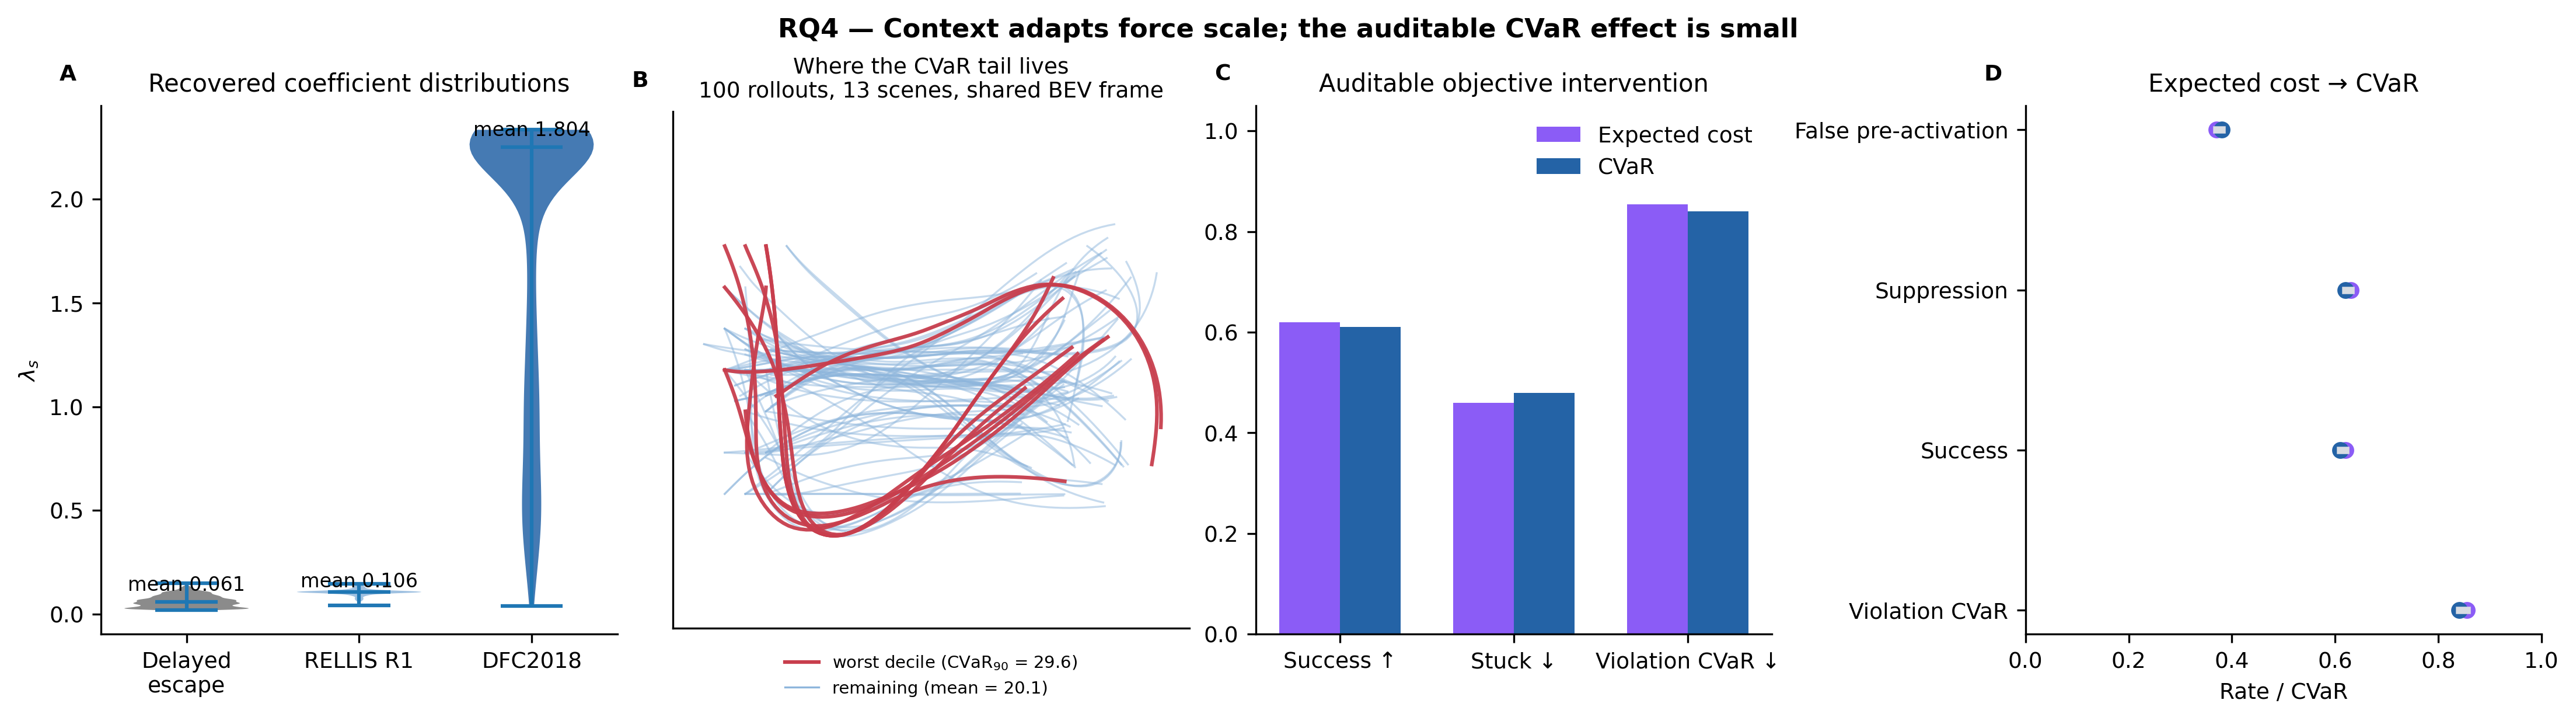
\includegraphics[width=\textwidth]{figures/rq4_adaptation_and_cvar.png}
\caption{\textbf{(RQ4) Context rescales the force across domains; the auditable
CVaR effect is small.}
\emph{A.} recovered $\lambda_s$ distributions, with mean $0.061$ on the
delayed-escape checkpoint, $0.106$ on RELLIS R1, $1.804$ on DFC2018, a
${\sim}30\times$ range from one model with no per-domain retuning. (These are
rollout-level samples; the point-level distribution means in
Table~\ref{tab:one_factor} are $0.107$ and $1.813$.)
\emph{B.} the CVaR tail located spatially, showing all $100$ logged rollouts in the
shared BEV frame, with the worst decile by path-integrated risk exposure in red
(CVaR$_{90}=29.6$ vs.\ mean $20.1$). The tail is made of long, doubling-back
routes. The $100$ episodes span $13$ scenes with differing event geometry, so
no field is drawn behind them.
\emph{C--D.} expected-cost vs.\ CVaR training on the same architecture and gate.
No metric separates the two arms at $95\%$ confidence over $100$ paired
episodes (Table~\ref{tab:delayed_escape}).}
\label{fig:rq4}
\end{figure*}

\begin{figure*}[htbp]
\centering
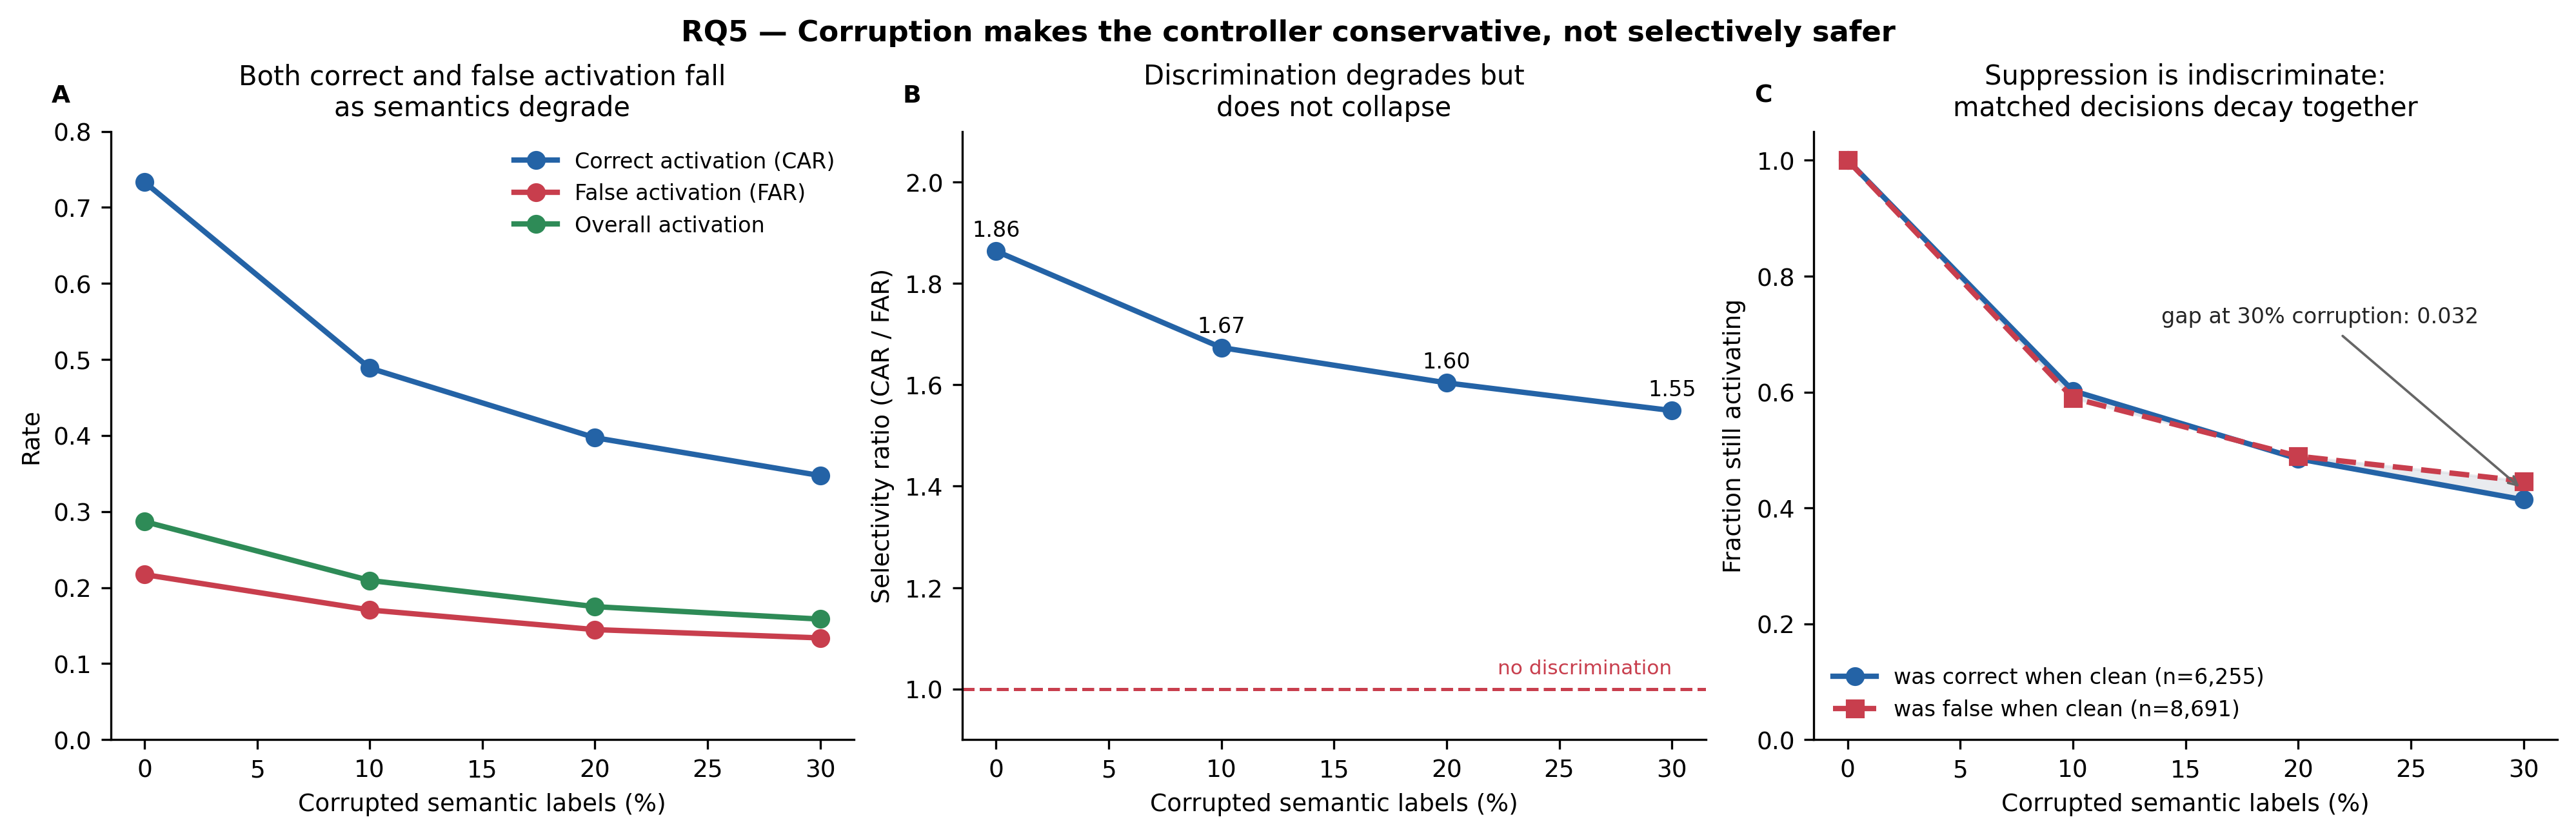
\includegraphics[width=\textwidth]{figures/rq5_perception_robustness.png}
\caption{\textbf{(RQ5) Semantic corruption makes the controller conservative,
not selectively safer.}
\emph{A.} correct- and false-activation rates both fall as semantic labels are
corrupted. \emph{B.} the selectivity ratio $\mathrm{CAR}/\mathrm{FAR}$ declines
from $1.86$ to $1.55$, so discrimination degrades but does not collapse to the
chance line at $1$. \emph{C.} the decisive test, over the $52{,}113$ decision
points matched across all four corruption levels. Activations that were
\emph{correct} on the clean map (${n}={6{,}255}$) and those that were
\emph{false} (${n}={8{,}691}$) decay almost identically, retaining $0.414$ and
$0.446$ at $30\%$ corruption, a gap of $0.032$. Corruption therefore
suppresses good and bad activations alike. Rates match
Table~\ref{tab:perception}.}
\label{fig:rq5}
\end{figure*}
